\documentclass[12pt, a4paper]{thesis}
\usepackage[a4paper, top=2.5cm, bottom=2cm, left=3.5cm, right=2.5cm]{geometry}

\makeatletter


\setcounter{secnumdepth}{4}
\setcounter{tocdepth}{4}
\usepackage{array}
\usepackage[T1]{fontenc}

\usepackage{subfigure}
\usepackage[utf8]{inputenc}  
\usepackage[T1]{fontenc} 
\usepackage{pdfpages}
\usepackage{bibtopic}
\usepackage{textcomp}
\usepackage{graphicx} %%For loading graphic files
\usepackage{fancyhdr} 
\usepackage{setspace}
\usepackage{amsmath,amssymb}
\usepackage[french]{babel}
\usepackage[french]{babel}
\usepackage[T1]{fontenc}
\usepackage{floatrow}
\usepackage{mwe}
\usepackage[dvipsnames]{xcolor}

\usepackage[latin1]{inputenc}
\usepackage{amsmath, amssymb}
\usepackage[latin1]{inputenc}
\usepackage[T1]{fontenc}
\usepackage[francais]{babel}
\usepackage{pdfpages}  
\usepackage[
  separate-uncertainty = true,
  multi-part-units = repeat
]{siunitx}


\frenchbsetup{StandardLists=true}
\usepackage{enumitem}
\usepackage{amssymb}
\usepackage{pifont}

\newcommand{\ts}[1]{\boldsymbol{#1}}
\newcommand{\vc}[1]{\boldsymbol{#1}}
\newcommand{\tsq}[1]{\mathbb{#1}}
\newcommand{\mtx}[1]{\mathbf{#1}}
\newcommand{\mvc}[1]{\mathbf{#1}}
\newcommand{\dd}[2]{\frac{\partial^2{#1}}{\partial{#2^2}}}
\newcommand{\dxy}[3]{\frac{\partial^2 {#1}}{\partial{#2}\partial{#3}}}
\newcommand{\ddx}[1]{\frac{\partial^2 {#1}}{\partial x^2}}
\newcommand{\dx}[1]{\frac{\partial{#1}}{\partial \vc{x}}}
\newcommand{\ddr}[1]{\frac{\partial^2 {#1}}{\partial r^2}}
\newcommand{\sig}{\ts{\sigma}}
\newcommand{\eps}{\ts{\epsilon}}
\newcommand{\dr}{\partial}
\newcommand{\veps}{\varepsilon}
\renewcommand{\arraystretch}{2}
\newcommand{\dt}{\Delta t}
\newcommand{\U}[1]{\{\itshape{U_{#1}}\}}
\newcommand{\dU}[1]{\{\itshape{\dot{U}_{#1}}\}}
\newcommand{\ddU}[1]{\{\itshape{\ddot{U}_{#1}}\}}

\usepackage[section]{placeins}

\usepackage{array,multirow,makecell}
\setcellgapes{1pt}
\makegapedcells
\newcolumntype{R}[1]{>{\raggedleft\arraybackslash }b{#1}}
\newcolumntype{L}[1]{>{\raggedright\arraybackslash }b{#1}}
\newcolumntype{C}[1]{>{\centering\arraybackslash }b{#1}}

\newcommand\eg{e.g.\ }

\renewcommand{\thesection}{\Roman{section}}
\renewcommand{\baselinestretch}{1.5}
\pagestyle{fancy}
\rhead{}
\lhead{\leftmark}
\pagestyle{fancy} 
\fancyhf{}            
\rhead{\thepage}

\renewcommand{\headrulewidth}{0.4pt}






\begin{document}


booootiiii555555aaaa



\newpage
\vspace*{100\p@}
\pagestyle{fancy}
\pagenumbering{roman}
\vspace*{10\p@}

\vspace*{10\p@}

\begin{center}
\section*{DÉDICACE}
\addcontentsline{toc}{section}{DÉDICACE}
\end{center}
\vspace*{40\p@}
\begin{center}

\textbf{\textit{
À ma chère mère Mounsa ma raison de vivre, qui éclaire mon chemin\\
À mon Père Jamel qui m'a toujours poussé et motivé\\
À mon fiancé Slouma, l'homme de ma vie. \\
À mes chères sœurs .. mes amours..\\
À mon cher frère Ayoub.\\
À mes anges Jad et Bayya.\\
À mon grand-père, qui j'adore.\\
À ma belle grande-mère.\\
À ma deuxième famille, la famille Salem\\
Rien ne saurait exprimer l’amour et le respect que j’ai toujours eu pour vous\\
}}
\end{center}
\vspace*{100\p@}


\newpage
\vspace*{10\p@}
\begin{center}

\section*{REMERCIMENTS}
\addcontentsline{toc}{section}{REMERCIMENTS}

\end{center}
\vspace*{20\p@}

\textbf{\textit{
Merci DIEU…\\} }

\textbf{\textit{
Ce projet est le résultat d’un travail de plusieurs mois durant lesquels j’ai pu bénéficier de nouvelles connaissances et compétences. Évidemment, ce projet est personnel, mais beaucoup de personnes y ont largement contribué de près ou de loin à la réalisation de ce travail.\\} }

\textbf{\textit{
En tout premier lieu, je tiens à remercier sincèrement Mme Ikram Zaag, M. Salem Fantar et M. Ahmed Labaied , en tant qu'encadrants professionnelles, qui ont facilité mon intégration au sein de SARTEX et se sont toujours montrés à l'écoute et ont fait preuve d'une disponibilité hors du commun tout au long de la réalisation de ce projet malgré leurs emplois du temps chargé. Je tiens à mentionner le grand plaisir que j'ai eu à travailler avec eux et avec toute l’équipe Six Sigma.\\} }

\textbf{\textit{
Je tiens à exprimer mes sincères remerciements à mon encadrant universitaire Pr Hassen Taleb, qui un enseignant et expert en Six Sigma pour son effort énorme, ces remarques qu’ont été précis et clairs, et pour ces conseils qu’il m’a accordée. Il me facilite grandement la tâche.\\} }

\textbf{\textit{
Il serait inconcevable de ne pas remercier le corps enseignant de l'école supérieure de la statistique et de l'analyse de l'information, qui ont largement participe à ma formation. Sans oublier tous les enseignants qui m'ont accompagné depuis le début de mon éducation.\\}}

\textbf{\textit{
Enfin, j'adresse mes vifs remerciements aux membres du jury qui me font l'honneur d'évaluer et de juger ce travail.\\}}

\addtocontents{toc}{\protect\thispagestyle{fancy}}

\tableofcontents
\listoffigures
\addcontentsline{toc}{section}{Table des figures}
\listoftables
\addcontentsline{toc}{section}{Liste des tableaux}

\begin{center}
\chapter*{liste des abréviation}
\addcontentsline{toc}{section}{Liste des abréviation}
\vspace{0.5cm}
\end{center}
 5M : Matières, Matériels, Milieu, Méthodes, Main-d'œuvre\\
 6$\sigma$ : Six Sigma\\
 AMDEC : Analyse des Modes de Défaillance, de leurs Effets et de leur Criticité\\
 BOM : Bill Of Materials\\
 CD : Cycle Développement\\
 DMAIC(S): Define (Définir), Measure (Mesurer), Analyze (Analyser), Improve (Améliorer), Control (Contrôler)\\
 IT : intervalle de tolérance. \\
 IPR : Indice de Priorisation des Risques.\\
 PPM : Pièces défectueuses Par Million. \\
 SKU : Unité de gestion des stocks.\\
 SMART : Spécifique ,Mesurable, Atteignable, Réaliste, Temporellement défini.\\
 VOC : Voice Of Customer (Voix du Client).\\
LSS : Lean Six Sigma\\
 




\thispagestyle{fancy}
\thispagestyle{fancy}
\newpage
\thispagestyle{fancy}
\pagenumbering{arabic}
\setcounter{page}{1}



\newpage
\begin{center}
\section*{INTRODUCTION GÉNÉRALE}
\addcontentsline{toc}{section}{INTRODUCTION GÉNÉRALE}
\vspace{0.5cm}
\end{center}


\newpage
\chapter{Cadre du projet}
\lhead{\leftmark}
\section*{Introduction}
\addcontentsline{toc}{section}{Introduction}

Dans le présent chapitre nous exposant le cadre du projet, nous allons présenter l’établissement d’accueil SARTEX, son domaine d’activité, sa structure organisationnelle et son processus de fabrication en général.\\
En deuxième lieu, on va détailler la problématique et les besoins suite auxquels ce projet a été créé.



\vspace{-0.5cm}
\section{Présentation de la société d'accueil}
\subsection{Présentation général}

\textbf{SARTEX}, abréviation de \textbf{« société des arts textiles »}, est une société privée tunisienne située dans la zone industrielle de Ksar Hellal. C’est une entreprise totalement exportatrice régie par la loi n°72/38 du 04/08/1972, spécialisée dans la confection, délavage et teinture d’articles variés pour hommes, femmes et enfants : pantalons, jackets, sports ‘wear’, jeans ‘wear, etc. 

\textbf{SARTEX} est le siège administratif de trois autres sociétés dans le même secteur d’activité qui sont :
\item - ELNOUR : Magasin de réception et de stockage de la matière première. Elle comprend également une unité de coupe.
\item - SOPAH : société spécialisée dans la confection textile.
\item - TEXPRO : société spécialisée dans la confection textile.

\\ \textbf{SARTEX} est mise en production depuis 1983. Sa capacité de production annuelle est de 3.5 millions articles pour une gamme de clientèle internationale dont principalement à l’instar de Hugo Boss, Polo Ralph Lauren, Guess, Lacoste… Ainsi qu’un effectif de 3500 employés. Elle occupe une surface actuelle de 17490 m².

\subsection{Organigramme de SARTEX}

\textbf{SARTEX} est une entreprise bien hiérarchisée. Son organisation est constituée d´une direction générale, des cadres, des agents de maîtrise et des agents d´exécution.
Elle dispatche ses activités entre les services, nous présentons un bref aperçu de l'organigramme de SARTEX (Fig. 1.1).
Notre projet a été effectué principalement au département Qualité. Ce service détecte, identifie et résout les problèmes de non-conformité lies à la qualité. Le responsable de qualité doit gérer et exploiter les informations relatives à la qualité sur des fiches. Le département qualité est lié à tous les ateliers, de la coupe jusqu´au délavage et conditionnement.

\begin{figure}[!h]
\begin{center}
        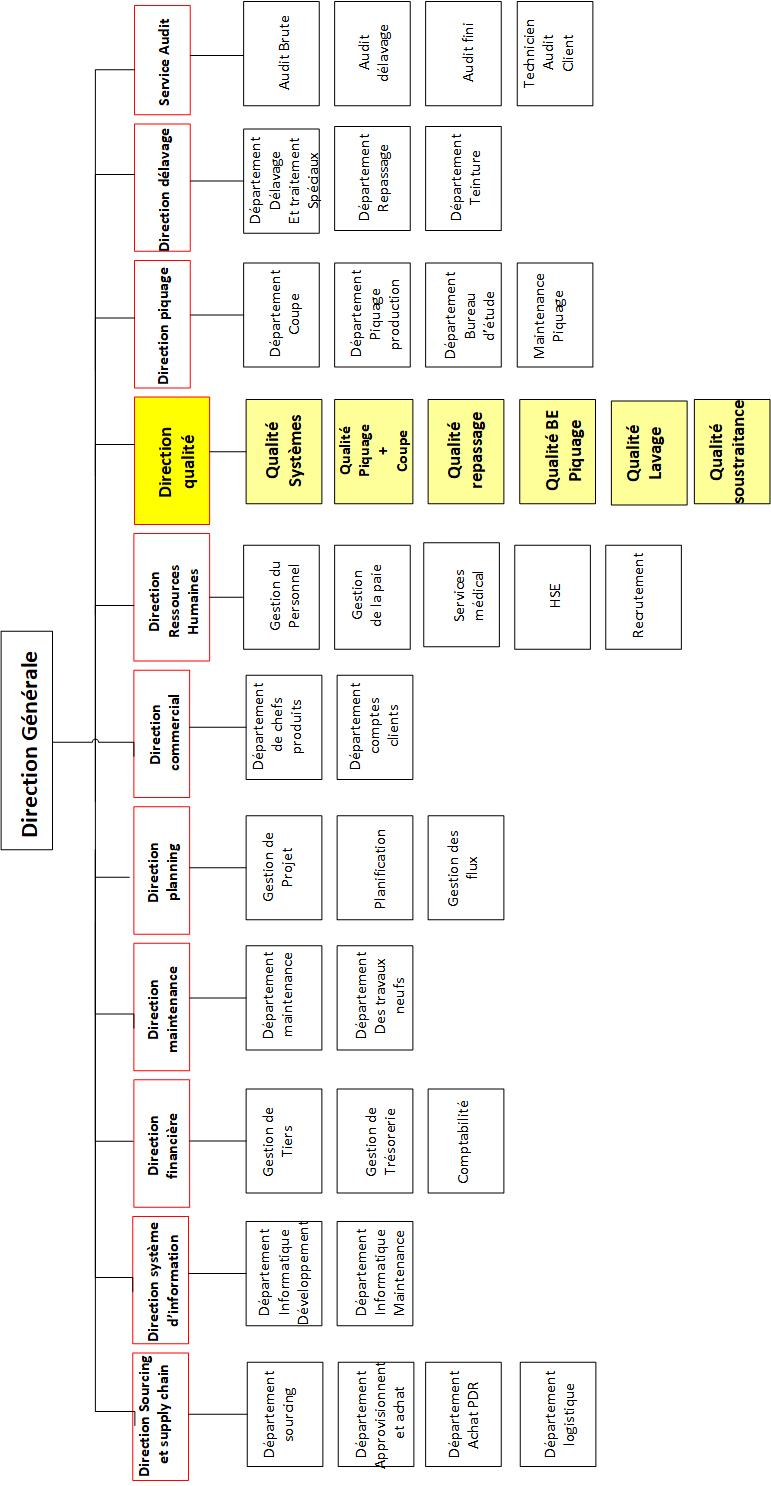
\includegraphics[scale=0.6]{orga.jpg}
        
        \caption{Organigramme de SARTEX}
\end{center}
\end{figure}


\subsection{Les différents ateliers}
Au sein de SARTEX il existe plusieurs ateliers.\\
\textbf{Atelier de coupe:}\\ où ils effectuent les opérations de placement, traçage et découpe des pièces entrant dans la composition des vêtements.\\
\textbf{Atelier de confection:}\\ C´est l´emplacement de la fabrication des articles textiles par l´assemblage des pièces coupées.\\
\textbf{Atelier de teinture:}\\ 
Dans cet atelier, on trouve deux laboratoires : un de recherche pour trouver une formulation des recettes des échantillons standards demander par les clients, et un deuxième laboratoire semi-industriel où il procède à une fixation de la recette industrielle.\\
\textbf{Atelier de délavage:}\\
Ce département comporte principalement deux unités : \\
• Le laboratoire de développement et la recherche : présente la base de tout le travail dans ce département. Sa fonction est le développement des recettes de délavage afin d´établir les différentes opérations nécessaires pour préparer les articles.\\
• L´atelier de production.\\
\textbf{Atelier de traitements spéciaux:}\\Afin d´avoir un produit fini et noble, on est amené à appliquer des traitements pour améliorer l´aspect de l´article comme le brossage, le spray, le sablage, moustache...\\
\textbf{Atelier de repassage et de contrôle final}:\\Le repassage est une étape finale lors de la fabrication des articles textiles qui est accompagné d´un contrôle final pour garantir une bonne qualité.\\ Après cette étape les articles seront transportés dans le magasin de stockage.\\ 

\subsection{Procédure de travail}
\subsubsection{Phase développement }
Généralement, le travail dans l’entreprise commence suite à une demande de client pour réaliser un nouveau produit. 

Une fois la demande est reçue, le chef produit en collaborant avec son assistant, préparent un statut interne de suivi indépendant pour chaque client et informe les autres parties concernées. Après la réalisation de la demande de développement, le chef produit s’occupe de l’identification des besoins en tissu, en fourniture, en accessoires et en traitements appliqués pour assurer la réalisation du prototype qui va être envoyé au client et qui passe par plusieurs étapes.
Dans le cas où le client refuse le prototype, le chef produit peaufine un autre jusqu’à l’accord du client en tenant compte de ses réclamations. Une fois le prototype est prêt, on commence la préparation d’une \textbf{COLLECTION} qui va suivre les mêmes étapes que ce dernier. Elle sera par la suite envoyée au client. Après confirmation, on passe à l’étape \textbf{« SIZE SET »} pour l’ajustement final des mesures et parfois pour quelques indications exigées par le client. Si elle est validée par le client, le processus de développement sera achevé par le lancement du chef produit qui signifie le déclenchement de la production en masse. 

\subsubsection{Phase production}
La production passe par une étape très importante qui est l’industrialisation appelée « Machine Test ». Selon la recette d’industrialisation, le chef production lance une première machine test contenant en moyenne 100 pièces pour bien fixer les écarts acceptables de traitement réalisé qui seront validés par la suite par le chef produit et après, ils lancent la production réelle.





\section{Problématique et objectifs}
Ce projet vise à maîtriser la qualité du processus de fabrication dans le but de baisser le nombre de défauts et le nombre de réclamations clients. En fait, les produits passent par plusieurs étapes de traitement, plusieurs caractéristiques de la qualité des produits font l’objet de réclamations des clients, ce qui est à l’origine de pertes importantes pour l’entreprise.\\
Parmi ces caractéristiques, les mesures dimensionnelles qui représentent un grand problème lorsque les limites de tolérances ne sont pas respectées, ce qui engendre un travail supplémentaire pour retravailler les pièces non-conformes. La mesure obtenue du produit fini dépend de plusieurs facteurs et des étapes de la production et phases et éléments du processus. La maîtrise de processus de production à un impact significatif et positif sur la variabilité de la qualité du produit fini et sur la satisfaction du client.\\
Donc l’entreprise SARTEX vise à développer et mettre en place un projet d’amélioration de la qualité des processus de production à fin de réduire la variabilité et par la suite la proportion de pièces non-conformes et le nombre de réclamations client.













\vspace{-0.3cm}
\chapter{Les méthodologies d'amélioration de la qualité }
\lhead{\leftmark}
\section*{Introduction}
\addcontentsline{toc}{section}{Introduction}
Dans ce chapitre, on va exposer les différentes méthodologies d'amélioration de la qualité brièvement et on va présenter aussi leurs historiques et les causes que donnent naissance à chaque méthodologie. Par la suite, on va comparer entre eux.\\


\section{Six Sigma}
Bill Smith \footnote{ ingénieur, 1929 – 1993} est un ingénieur chez Motorola introduit en 1986 le terme de Six Sigma comme réponse à un objectif de production « \textbf{sans défaut }». Six Sigma est donc une méthode d'\textbf{amélioration de la qualité} et de l'efficacité des processus.. Motorola est la première société utilisant le Six Sigma comme outil d'amélioration de la qualité pour ses produits électroniques.

Un autre personnage-clé dans le développement de Six Sigma est Mikel Harry\footnote{fondateur de l'Académie Six Sigma en 1994}, définit les bases de $6\sigma$ s’appuyant sur la philosophie de William Edwards Deming\footnote{ statisticien, 1900 - 1993} (roue de la qualité) et qui a aussi attribué avec la convention de nommage de Ceintures Noires (Black Belts) et ceintures vertes (Green Belts), ce sont les chefs de projet avec divers niveaux de compétence de Motorola.

La philosophie Six Sigma va ensuite se développer et se perfectionner dans les années 90 sous la houlette de grandes sociétés américaines, avec en-tête de proue General Electric. [9]




\section{Lean manufacturing}
En 1950, Toyota est au bord de faillite donc elle doit impérativement réduire ses coûts et améliorer son efficacité.  OHNO\footnote{ ingénieur industriel japonais chez Toyota, 1912 - 1990} se rend aux Etats-Unis pour étudier les lignes de montage de Ford.De retour du Japon, il met au point le Système de Production Toyota (TPS), considéré depuis comme le meilleur modèle de production au monde et le précurseur du Lean Manufacturing.


Au moment même où T. Ohno et son équipe développaient le nouveau système de production de Toyota, le constructeur ne vendait pas un seul modèle en quantités suffisantes pour justifier la mise en œuvre des techniques de production en série de Ford. En outre, il ne pouvait pas se permettre un investissement dans les équipements complexes réputés être la clé de l’amélioration de la productivité. \\ 

T. Ohno définit alors sept catégories de gaspillage ou 7 Muda :
\item 1. Production excessive .
\item 2. Attentes : attendre des pièces ou une machine qui finit son cycle.
\item 3. Transports et manutentions inutiles.
\item 4. Usinages inutiles : toutes opérations non strictement nécessaires contribuant à dépasser les attentes du client et mobilisant des ressources.
\item5. Stocks excessifs .
\item 6. Mouvements inutiles.
\item 7. Défauts et rebuts\\

T. Ohno et son équipe se sont donc évertués à éliminer les pertes de temps et les activités inutiles à chaque étape du processus de production, parvenant au final à réduire considérablement les coûts et les délais de production. Ils ont également mis au point un processus novateur pour changer rapidement les équipements, afin de produire différents modèles.

Le Système de production Toyota a permis à ce constructeur de produire des véhicules en continu, bien plus rapidement et efficacement que ses concurrents, ce qui lui a conféré un avantage déterminant.\\



\section{Lean Six Sigma}
Lean Six Sigma est une combinaison entre le Six Sigma et Lean. \\
D'une part, le concept Lean a pour objectif d’éliminer tous les tâches inutiles, sans valeur ajoutée. Lean vise aussi à simplifier les processus en augmentant la fluidité, la flexibilité, l’agilité et ce dans un objectif d’accroître la valeur pour le client et de contribuer à l’amélioration des performances de l’entreprise. De l'autre part le concept Six Sigma vise à améliorer la qualité et reduire le nombre des défauts.\\
Donc cette combinaison relie entre la qualité et la productivité en se basant sur ces 5 principes pour rendre son application efficace :
\item - Loi du marché : « Les besoins du client définissent la qualité et sont la plus haute priorité de l’amélioration ».
\item - Loi de la flexibilité : « La vitesse de n’importe quel processus est proportionnelle à sa flexibilité (c’est-à-dire, la facilité avec laquelle les gens peuvent passer d’une tâche à l’autre.».
\item - Loi de la concentration : « Les informations montrent que 20\% des activités au sein d’un processus causent 80\% des problèmes et des retards ».
\item - Loi de la vitesse : « La vitesse de tout processus est inversement proportionnelle à la quantité de travaux en cours »
\item - Loi de la complexité et du coût : « La complexité d’une offre de service ou du produit ajoute généralement plus de coûts et des travaux en cours que ne le font des problèmes de qualité (sigma peu élevé) ou de lenteur (contraire de Lean) ».\\



\begin{figure}[!h]
\begin{center}
        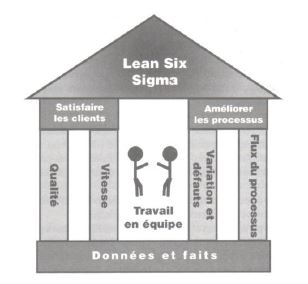
\includegraphics[scale=0.7]{LSS.JPG}
        
        \caption{LSS: Lean Six Sigma}
\end{center}
\end{figure}






\section{Comparaison entre les différents méthodologies }
La différence fondamentale entre le Lean et le six sigma est que le Lean se concentre sur l'élimination des déchets alors que le six sigma, lui se focalise sur l'élimination des variations.\\
Dans le monde de la production industrielle, le Lean est l'application du juste-à-temps(JAT).Les matières premières arrivent que quand on en a réellement besoin, c'est le principe du "flux tendu". Cela a comme objectif de réduire au maximum les stocks et les encours. Pour optimiser les performances, les matières premières doivent être déchargées et acheminées sur les lignes d'assemblage le plus rapidement et suivant la trajectoire le plus courte possible.\\
Le but du Lean manufacturing est d'éviter d'avoir à l'entrée beaucoup de matières premières qui attendent à être utilisées et avoir à la sortie une quantité de produits allant au-delà de ce que les clients ont commandé.
Alors que l'objectif de Six Sigma est d'avoir à la sortie des produits finis qui sont cohérents et sans défauts : c'est d'élimination les variations \\  En effet, les produits finis défectueux nécessitent un travail supplémentaire qui constitue un déchet. Les produits finis incohérents sont souvent le résultat d'un processus de production défectueux. Le Six-Sigma vise donc à identifier les défauts, en déterminer la cause, et à les éliminer. Comme exemple, supposons que l'on a une usine qui fabrique des objets connectés.\\
Ces objets connectés sont tous censés être d'une certaine taille/forme/poids. A la fin de production, vous découvrez que sur 1.000 objets connectés, 50 sont imparfaits (mauvaise taille, forme, ou poids). Pour corriger cela, vous pouvez utiliser le Six-Sigma pour déterminer ce qui cause ces variations / défauts et travailler à les réduire à un niveau de six sigma.\\
Bien qu'il peut être souhaitable d'utiliser à la fois le Lean et le Six-Sigma, ce sont deux méthodologies qui répondent à des questions distinctes : un processus peut être Lean et avoir un taux élevé de variation à la sortie. Ce même processus peut aussi avoir une variation sous contrôle et ne pas être Lean. Les deux méthodologies sont donc complémentaires et indépendantes. [10] \\ 

































\vspace{-0.3cm}
\chapter{Méthodologie Six Sigma}
\section{Concept Six Sigma}
\subsection{Définition et base statistique}
Le Six Sigma est une méthode, orientée qualité, vise à optimiser les processus de fabrication en vue de satisfaire les clients et se base sur une démarche fondée à la fois sur la voix du client et sur des données mesurables (indicateurs, etc.) et fiables.\\
Cette méthode est utilisée dans des démarches de réduction de la variabilité dans les processus de production (ou autre) et au niveau des produits et vise ainsi à améliorer la qualité globale du produit et des services. \\
Un processus industriel comprend un certain nombre de tâches répétitives, l'exemple le plus caricatural étant la production d'une pièce en grande série. Une pièce est conforme si elle respecte un certain nombre de critères, cependant, toutes les pièces produites ne peuvent pas être strictement identiques. Une des préoccupations majeures de la gestion de la qualité est donc de maîtriser les conditions de production afin qu'il y ait le moins de \textbf{rebut}, le moins d'insatisfaction client possible. \\
Les rebuts sont les produits hors de l’intervalle de tolérance IT, qui sont représentés sont les parts de l’échantillon aux extrémités de courbe d’une dispersion normale illustré en bleu sur la Fig. 3.1
\begin{figure}[!h]
\begin{center}
        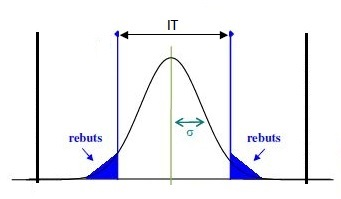
\includegraphics[scale=1]{IT.JPG}
       \caption{La dispersion normale et les rebuts}
\end{center}
\end{figure}
Avant que le terme de six sigma ne devienne le nom de la méthode, il était une simple référence statistique à la courbe de Gauss (ou loi normale) qui précise la dispersion d’une série de données autour de la moyenne. Six Sigma signifie donc « six fois l’écart type », c’est pour atteindre un niveau d'excellence et parler d’une exceptionnelle absence de défaut.
\begin{table}[!htbp]
\begin{center}
\baselin eskip 20pt
\begin{tabular}{|C{5cm}|C{6cm}|C{3cm}|} 
\hline 
\textbf{Limites de spécification} & \textbf{Pourcentage de conformité}  & \textbf{PPM}\\ 
\hline 
\textbf{\SI{\pm 1 }$\sigma$} & 68.27 \% & 317300\\
\hline 
\textbf{\SI{\pm 2 }$\sigma$} & 95.45 \% & 45500 \\ 
\hline 
\textbf{\SI{\pm 3 }$\sigma$} & 99.73\% & 2700 \\ 
\hline 
\textbf{\SI{\pm 4 }$\sigma$} & 99.9937\% & 63 \\ 
\hline 
\textbf{\SI{\pm 5 }$\sigma$} & 99.999943\% & 0.57 \\ 
\hline 
\textbf{\SI{\pm 6 }$\sigma$} & 99.9999998\% & 0.002 \\ 
\hline 
\end{tabular} 
 \caption{Les niveaux 6 Sigma}
 \end{center}
\end{table}


\subsection{La relation entre la capabilité processus et Six Sigma}


La notion de Six Sigma et la capabilité sont deux notions inséparables. \\
La capabilité est la mesure traduisant le rapport entre la performance réelle d'un processus et la performance cible. Elle permet de mesurer l'aptitude d'un processus à réaliser des pièces conformes aux spécifications imposées par le cahier des charges. Le fait d'utiliser un chiffre pour caractériser la capabilité est fondamental.

L'étude de capabilité de processus est une technique essentielle dans l'analyse des données. On peut l'utiliser pour tous les types de données obtenues à partir d'un processus de production. Toutefois, l'étude de capabilité du processus est d'abord une technique de recherche, et à ce titre elle est particulièrement importante dans tous les domaines de l'ingénierie.

La capabilité se définit comme étant l'intervalle de tolérance divisé par 6 fois l'écart type de la distribution du processus en question, notée Cp\\
\textbf{\[Cp=\frac{IT}{6\sigma } ~~~~~~~~ (1)\]}



Selon les valeurs de capabilité on distingue plusieurs cas : 

Si \textbf{\underline{Cp<1}} : notre processus est non capable, il existe un nombre non-négligeable d'observation en dehors de IT c'est très insuffisant.\\

\begin{figure}[!h]
\begin{center}
        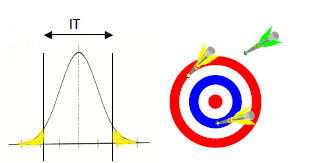
\includegraphics[scale=1]{noncapable.png}
        
        \caption{Processus non capable}
\end{center}
\end{figure}\\

Si \textbf{\underline{Cp=1}} : on peut dire que notre processus est juste capable, mais il faut faire attention.
\begin{figure}[!h]
\begin{center}
        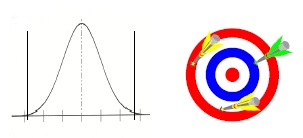
\includegraphics[scale=1]{justecapable.jpg}
        \caption{Processus juste capable}
\end{center}
\end{figure}\\


Si \textbf{\underline{Cp>1.33}} : notre processus est capable, c’est suffisant.\\
\begin{figure}[!h]
\begin{center}
        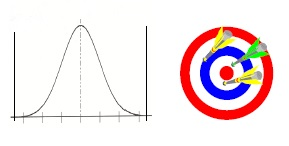
\includegraphics[scale=1]{capable.jpg}
        
        \caption{Processus capable}
\end{center}
\end{figure}\\
Parmi les cas possibles que le processus est décentré et la dispersion autour de la moyenne est faible, dans ces cas la moyenne est différente à la moyenne théorique. Cette différence est exprimée par le facteur de décentrage est noté par \textbf{k} (Fig. 3.5).\\
\begin{figure}[!h]
\begin{center}
        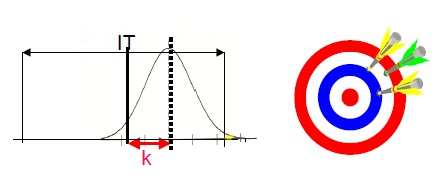
\includegraphics[scale=0.85]{centr.jpg}
        \caption{Processus décentré}
\end{center}
\end{figure}\\
Par conséquent, on peut observer des rebuts à l’un des deux côtés de \textbf{IT}. Si on tient compte de ce décentrage, on peut alors définir un nouvel indicateur, c’est l’\textbf{indicateur de réglage}, noté \textbf{Cpk}:

\[Cpk=\frac{IT - 2k}{6\sigma}  ~~~~~~~~  (2)\]  

À long terme il est impossible détecter ou d’observer un décentrage de moins de 1.5 sigma, donc il faut introduire une "correction" de 1,5 $\sigma$ dans le calcul :\\
6$\sigma$ - 1,5$\sigma$ = 4,5$\sigma$ (Fig 3.6)
\begin{figure}[!h]
\begin{center}
        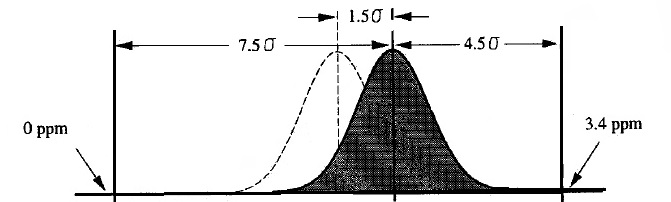
\includegraphics[scale=0.75]{v1.jpg}
        \caption{Processus décalé à long terme }
\end{center}
\end{figure}
\\Et par la suite le processus Six Sigma admet 3,4 pièces défectueuses par million (PPM) au lieu de 0.002 PPM, alors on obtient une nouvelle table des niveaux 6 sigma avec un décalage de 1,5 $\sigma$.\\
\begin{table}[!htbp]
\begin{center}
\baselineskip 20pt
\begin{tabular}{|C{5cm}|C{6cm}|C{3cm}|} 
\hline 
\textbf{Limites de spécification} & \textbf{Pourcentage de conformité}  & \textbf{PPM}\\ 
\hline 
\textbf{\SI{\pm 1 }$\sigma$} & 30.23 \% & 697700\\
\hline 
\textbf{\SI{\pm 2 }$\sigma$} & 69.32 \% & 608700 \\ 
\hline 
\textbf{\SI{\pm 3 }$\sigma$} & 93.32\% & 66810 \\ 
\hline 
\textbf{\SI{\pm 4 }$\sigma$} & 99.3790\% & 6210 \\ 
\hline 
\textbf{\SI{\pm 5}$\sigma$} & 99.97670\% & 233 \\ 
\hline 
\textbf{\SI{\pm 6}$\sigma$} & 99.999660\% & 3.4 \\ 
\hline 
\end{tabular} 
 \caption{Les niveaux 6 Sigma avec décalage de 1.5 Sigma}
 \end{center}
\end{table}\\
Pour conclure la méthodologie Six Sigma représente l’objectif « idéalisé » d’un taux de défauts de 3,4 produits défectueux sur un échantillon d’1 million, ce qui correspond à un taux de qualité de 99,9997 \%.\\
Il faut cependant garder à l’esprit que l’objectif final de la méthode Six Sigma n’est pas d’atteindre la perfection, mais un niveau de qualité acceptable par les clients.

Outre le fait que le niveau de qualité est meilleur, la nouveauté est d’appliquer la méthode à tous les processus de l’entreprise : faciliter la prise de commande du client, diminuer le temps de livraison…\\
En somme, l’application de la méthode Six Sigma permet :
\item• La réduction des dépenses en diminuant le nombre de rebuts, de retraitements et de gaspillages ;
\item• L’optimisation de l’utilisation des équipements de l’entreprise ;
\item• L’augmentation de la satisfaction des clients ;
\item• L’augmentation du chiffre d’affaires grâce à la réduction des coûts et à l’amélioration de la qualité.

\section{Cycle Six Sigma: DMAIC}
Les projets Six Sigma passent par une séquence d’étapes standard connue sous le nom de DMAIC (Définir, Mesurer, Analyser, Innover, Contrôler) qui vont etre développée dans la suite de ce travail.\\

DMAIC est une méthode d’investigation expérimentale, analytique et scientifique exécutée en mode projet. C’est d’ailleurs la démarche que tout bon praticien (qu’il soit ingénieur ou charpentier) applique afin de résoudre durablement un problème. \\
Utiliser ce système permet de s’assurer que les ressources de l’entreprise sont utilisées à bon escient et que les équipes reçoivent le soutien dont elles ont besoin pour finaliser leurs projets à temps et dans la limite du budget, et aussi de réaliser les objectifs du Six Sigma (satisfaction clients, réduire le nombre des défauts...)

\begin{figure}[!h]
\begin{center}
        
\includegraphics[scale=0.4]{DMAIC1.png}
        \caption{Démarche DMAIC}
\end{center}
\end{figure}

\subsection{Phase DEFINIR}
Dans cette étape, on définit le problème, le périmètre du sujet que l'on souhaite traiter et de cibler l'objectif à atteindre par rapport aux attentes client. Autrement dit, c'est d'exprimer les symptômes douloureux ressentis par le client par exemple les coûts élevés, les défauts...

Il y a plusieurs outils pour cette phase DEFINE comme :

\subsubsection{Charte de projet}

Ce document sert à clarifier les différents éléments du projet et doit contenir les parties suivantes :

• Objectifs, bénéfices et exigences du projet.

• Première analyse des parties prenantes du projet.

• Signatures des parties prenantes clés.

• L'équipe projet et les coordonnées des membres.

• Le planning du projet.

• Les aspects financiers du projet, les gains escomptés et les dépenses.

La charte de projet est un document dynamique. On peut le modifier ou l'ajusté au cours du projet. Voir annexe ref{nour11111}.
\subsubsection{SIPOC}
Le SIPOC est l'acronyme de :
\item • Suppliers : sont les personnes qui fournissent informations, matériels, formulaires.. 
\item • Inputs : sont les matières premières ou les informations ou les matériels utilisés
\item • Process : sont les étapes du processus
\item • Outputs : sont les informations, le produit ou le service fournis au client
\item • Customers : l’étape suivante dans le processus ou le client final.\\
SIPOC est une carte de processus assez simple qui se penche sur le processus à un niveau relativement élevé. Il est un outil visuel pour documenter un processus d'affaires de bout en bout, ce qui est très utile au début d'un projet membres de l'équipe en aidant d'accord sur un langage commun et la compréhension de l'ensemble du processus.



\subsubsection{QQOQCP}
 Qui ? Quand ? Où ? Quoi ? Comment ? Combien ? Pourquoi ? Ce sont des questions dites « ouvertes » qui nécessitent une forme de réponse développée.
 
La méthode QQOQCP est un outil simple et fréquemment utilisé afin de faire le tour de l’ensemble d’un sujet qui apporte les informations qui permettent de mieux connaître, cerner, clarifier, structurer, cadrer une situation, car elle explore toutes les dimensions sous différents angles. 

Il peut aussi être utilisé pour définir les modalités de mise en œuvre d’un plan d’action. Il évite d’oublier un élément indispensable à la réussite du projet. \\
- \textbf{Qui} : pour déterminer les parties prenantes engagées.\\
$ \Longrightarrow$  Qui est le concerné ? Quelle personne ? Quel service ? Quel fournisseur ou client ? \\
- \textbf{Quand} : pour bien situer les choses dans le temps. \\
$ \Longrightarrow$ À quel moment ? Depuis quand ? Fréquence ? \\
-\textbf{ Où} : pour situer les choses dans l’espace. \\
$ \Longrightarrow$ À quel endroit ? À quelle étape ? Quel secteur ? Sur quel procédé ? \\
-\textbf{ Quoi} : pour mettre le focus sur un point précis. \\
$ \Longrightarrow$ Quel est le problème ? Quel produit ? Quel est le défaut ? Quelle quantité ?...\\
- \textbf{Comment} : pour connaître des étapes, des manières de procéder. \\
$ \Longrightarrow$ Comment a été détecté le problème ? Par quel moyen ? Quel matériel ? \\
- \textbf{Combien} : Expose le besoin de connaître un nombre ou une valeur.\\
$ \Longrightarrow$ Combien de temps ? Combien de fournisseurs ? Combien d’effectifs ?\\
- \textbf{Pourquoi} : chercher les informations pour expliquer les causes et les raisons. \\
$ \Longrightarrow$ Est-ce un problème ? Quel coût ? \\
En répondant à ces questions, l’équipe génère des idées qui seront notées et par la suite l’équipe définit l’objectif du projet concret et le plan d’action. 

\subsection{Phase MESURER}

L'objectif de la phase mesure est de collecter des données sur le terrain, représentatives de la situation actuelle, en passant par l'étape de la cartographie du processus (flux de processus).

Afin de mieux appréhender le processus et les causes racines du problème et en même temps dégager des tendances qui seront étudiées dans la phase ANALYSER (statistiques descriptives - diagramme de Pareto).

Il s'agit également de mesurer la performance de système de mesures (Gage R&R). Enfin, on pourra estimer la capabilité de processus (Cp, Pp, Cpk, Ppk).


\subsubsection{Flux de processus}

Un flux de processus est un outil de visualisation des étapes et des points décisionnels d’un processus métier. Il est souvent utilisé pour faciliter la compréhension du flux et identifier les opportunités d’amélioration (en connaissant les sources de variation, d’interruption et de gaspillage..). \\
Pour présenter les étapes, il faut utiliser des symboles bien spécifiques. (voir table 3.3)

\begin{table}[!htbp]
\begin{center}
\baselineskip 20pt
\begin{tabular}{|C{4cm}|C{3cm}|C{7cm}|} 
\hline 
\textbf{Symbole} & \textbf{Nom}  & \textbf{Description}\\ 
\hline 
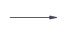
\includegraphics{connecteur.JPG} & Connecteur & Les flèches indiquent la direction d'organigramme \\
\hline 
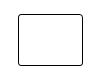
\includegraphics[scale=0.7]{etape.JPG} & Etape & représente une action, une tâche ou une opération qui doit être effectuée\\
\hline 
\end{tabular} 
 \end{center}
\end{table}\\
\begin{table}[!htbp]
\begin{center}
\baselineskip 20pt
\begin{tabular}{|C{4cm}|C{3cm}|C{7cm}|}
\hline 
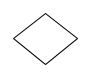
\includegraphics[scale=0.7]{dd.JPG} & Décision & Le point auquel une décision doit être prise. « oui » ou « non ».\\
\hline 

\includegraphics{df.JPG} & Terminator &	Représente les points d'entrée et de sortie de votre organigramme (il existe un seul point de départ, mais peut disposer de plusieurs points de fin\\
\hline 

\end{tabular} 
 \caption{Les symboles du flux de processus}
 \end{center}
\end{table}\\
\newpage
\subsubsection{Le diagramme de Pareto}
La loi de Pareto, appelée aussi  règle des 80/20, est un phénomène empirique révélant que 80 \% des effets sont le produit de 20\% des causes.\\
L’une de très célèbre exemple « 80\% des richesses détenues par 20\% de la population » qui analyse les données fiscales de différents pays par l’économiste italien \textbf{Vilfredo Pareto}\footnote{économiste italien, 1848 - 1923} qui mit ce principe en évidence pour la première fois au début du 20ème siècle.\\
Le diagramme de Pareto permet de définir des priorités dans le traitement des problèmes. Dans ce cas, 20\% de causes permet de résoudre 80\% du problème. Cette loi est donc utile pour définir sur quelles causes agir en priorité.
\begin{figure}[!h]
\begin{center}
        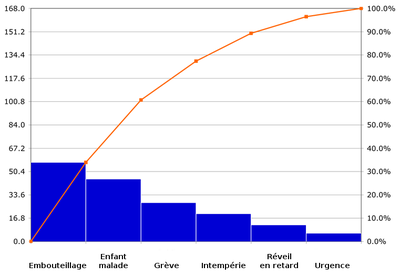
\includegraphics[scale=0.7]{diag.png}
        \caption{Exemple de diagramme de Pareto}
\end{center}
\end{figure}

\subsubsection{Performance de système de mesure (Gage R&R) }
Le Gage R&R, appelé aussi MSA (Measurement Systems Analysis), est un outil statistique de mesurer la performance d'un système de mesures permet de mesurer la Répétabilité et Reproductibilité de ce système : règle, pieds à coulisse, chronomètre... Afin de valider la méthode par laquelle on collecte les données.
Via ce test on peut calculer un pourcentage de variation totale du processus de mesure et par la suite, on peut qualifier le système de mesures.\\
\textbf{La reproductibilité} est la capacité d’un moyen à mesurer dans des conditions variables : opérateurs, appareillages, temps...\\
\textbf{La répétabilité} est l’évaluation des mesures d'un même échantillon dans presque ou faiblement variables : même protocole de mesure, même appareillage, même opérateur dans un faible intervalle de temps.\\
Analyse de résultats :\\
- Gage R\&R < 10\% : le système de mesures est bon.\\
- 10\% < Gage R&R < 30\% : le système de mesures est acceptable.\\
- Gage R\&R >30\% : le système de mesures n’est pas acceptable.\\
Et par la suite, on distingue deux situations:\\
Si la reproductibilité est mauvaise : cherchez du côté de la formation, des standards et de la définition.\\
Si la répétabilité est mauvaise : cherchez du côté de l’outil de mesure lui-même.\\




\subsection{Phase ANALYSER}
Il s’agit de chercher les causes de variabilité du processus en exploitant les données collectées dans la phase mesure.\\
Il existe deux divisions d’outils :
\item - Des outils de résolution de problèmes afin de dégager les causes racines de variabilité : méthode de 5W, diagramme d’Ishikawa, brainstorming, AMDEC …
\item – Des outils statistiques qui établirent les relations entre les paramètres d’entrées Xi et la variable réponse Y : les tests d’hypothèse, les tests de variance, les tests de normalité….





\subsubsection{Diagramme d’Ishikawa}

Le diagramme causes-effets d'Ishikawa est un outil qualité (graphique) utilisé pour identifier et étudier les causes potentilles d'un problème ou d’une situation constatée. 
Cette méthode est basée sur la recherche des causes liées à l’effet selon les 5 M (5 axes):\\
•	Matières : tout ce qui est consommable et utile au projet (Les entrées)\\
•	Matériels : les matériels de production et de suivi\\
•	Milieu : le contexte de travail \\
•	Méthodes : les techniques et procédures\\
•	Main-d'œuvre : le personnel \\


\begin{figure}[!h]
\begin{center}
        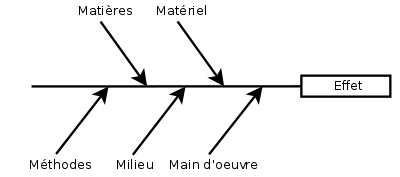
\includegraphics[scale=0.75]{chika.png}
        \caption{Diagramme d’Ishikawa}
\end{center}
\end{figure}


\subsubsection{Brainstorming}
Le brainstorming, littéralement, est une tempête de cerveaux, c'est une méthode de résolution de problèmes s'appuyant sur la créativité spontanée des participants. En fait, c'est bien la spontanéité qui est recherchée.\\
Le protocole de brainstorming en pratique :\\
Lors d'une session, toutes les idées sont notées sans n’y apporter aucun jugement. Au contraire, même il est plutôt demandé aux participants de ne pas critiquer, et de ne pas hésiter à rebondir pour construire et laisser progresser la réflexion. Ainsi, par association d'idées successives, on collecte de nombreuses pistes [12].\\

\subsubsection{l'AMDEC}
L'AMDEC est une méthode d'Analyse des Modes de Défaillance, de leurs Effets et de leur Criticité.\\
Cette méthode est une méthode qualitative d'analyse prévisionnelle, outil de gestion de la qualité applicable à un processus, à un produit, à un organisme ou à un délai. Elle est basée sur un raisonnement basée sur un raisonnement inductif visant à identifier les risques de pannes potentiels contenus dans un système pour les supprimer ou les maîtriser et par la suite améliorer la performance.[1]







\subsubsection{Test d'hypothèse}

Un test d'hypothèse est une procédure de décision permettant d'accepter ou de rejeter une hypothèse statistique (H0 : hypothèse nulle) avec une probabilité donnée.

Pour appliquer les tests d'hypothèse, il faut faire l'appel à un nombre d'hypothèses pour vérifier les conditions d'application et connaître la nature de la population étudiée (normalité de la variable, égalité des variances...).\\
Pour tester une hypothèse, il faut :

(1) Définir l'hypothèse nulle $H_{0}$

(2) Choisir un test statistique ou une statistique

(3) Définir la distribution de la statistique sous $H_{0}$

(4) Définir le niveau de signification du test $\alpha$

(5) Calculer la valeur de la statistique

(6) Prendre la décision





\subsection{Phase AMÉLIOER}

Après avoir dégagé les problèmes dans la phase analyse, la phase amélioration consiste à chercher des solutions afin de réduire les variabilités du processus. Il s’agit de trouver une ou plusieurs solutions appropriées pour chacune des causes des défauts ou de variabilité. \\
Les solutions pourront être classées grâce à une matrice enjeux/accessibilité et mettre en place les actions retenues relatives.\\
Cette phase est basée sur différents outils : plan d'expérience, Benchmarking, les 5 M, les tests d'hypothèse, AMDEC.. 

\subsubsection{Plan d'expériences}
Les plans d'expériences, connus sous l'appellation DOE (Design Of Experiment), c'est un outil statistique efficiente et efficace de la relation cause-effet entre certaines variables du processus (les facteurs) X et la variable réponse Y.

Le plan d'expériences identifie les sources majeures de variation (X) celles qui ont l'impact le plus important sur les résultats. Il quantifie aussi les effets des X importantes, y compris leurs interactions. On obtient une fonction du type :
\begin{center}
$Y=f(X)$
\end{center} 
Cette approche est très optimale, utilisée généralement dans des recherches scientifiques ou des études industrielles afin de découvrir le maximum des nouvelles reconnaissances avec le minimum d'expériences.

Pour réussir cette méthode, il faut suivre les étapes suivantes :\\
– Choisir les caractéristiques à mesurer. \\
– Identifier les facteurs à tester. \\
– Créer une matrice d’expériences.\\
– Réaliser les expériences et noter les résultats dans la matrice d’expériences.\\
– Analyser les résultats et tirer des conclusions. \\
– Faire un essai de validation des résultats finals.\\


\subsection{Phase CONTROLER}


Après avoir trouvé des solutions et les appliquer, il ne reste qu’à suivre l’évolution de la nouvelle situation et à maintenir les changements. Au fur et à mesure mesurer l’efficacité des solutions à long terme.\\
Les outils à employer dans cette étape sont plusieurs : les cartes de contrôle, Kaizen, Gage R\&R, Diagramme de Pareto, Poka-Yoké…


\subsubsection{Kaizen}
Kaizen est un processus d'améliorations concrètes, simples et réalisable dans une période très courte sous forme de petites actions.\\
\begin{figure}[!h]
\begin{center}
        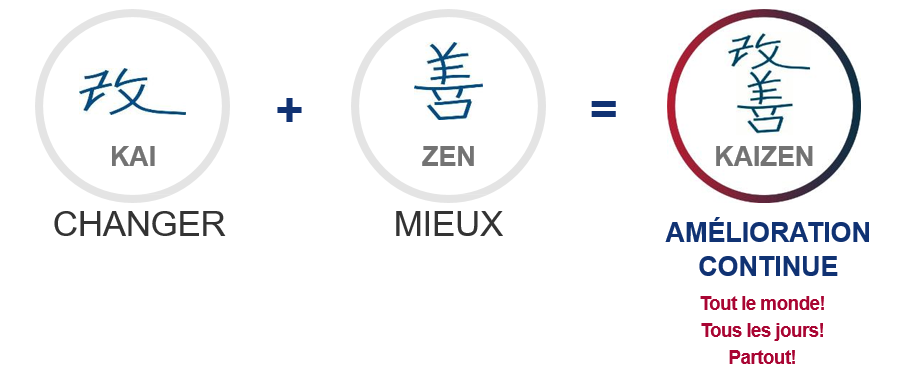
\includegraphics[scale=0.4]{kaizen.PNG}
        \caption{kaizen}
\end{center}
\end{figure}\\


L'idée n'est pas de lancer de grands projets et des investissements conséquemment, mais plutôt de motiver tout un chacun afin que la recherche de l'amélioration continue devienne un réflexe de tous les instants et de toutes les situations en fait cette phrase résume tout l'esprit de Kaizen:\textbf{"Fais le mieux, rend le meilleur, améliore  le même s'il n'est pas cassé, parce que si nous ne le faisons pas, nous ne pouvons pas concurrencer ceux qui le font"}.
 
\subsubsection{Poka-Yoké}
Le Poka-Yoké est une méthode sert à prévenir les erreurs et l’empêcher de se réaliser, autrement dit cette méthode vise à contrôler les erreurs et non pas les défauts. Elle est utilisée souvent dans les industries pour assurer la bonne qualité.\\
\begin{figure}[!h]
\begin{center}
        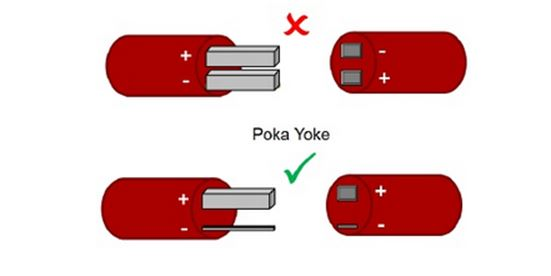
\includegraphics[scale=0.8]{poka.jpg}
        \caption{Exemple de Poka-Yoké}
\end{center}
\end{figure}\\
Démarche :\\
•	Identifier les personnes concernées par la problématique. \\
•	Identifier l’emplacement d’erreur.\\
•	Analyser le problème.\\
•	Chercher la solution convenable pour s’assurer que le problème ne se répète plus.\\
•	Vérifier le fonctionnement de la solution.\\


\subsubsection{Cartes de contrôle}
Une des actions les plus importantes pour aider à maintenir la qualité d'une fabrication ou d'un service est la collecte de données informatives de façon consistante dans le temps, la visualisation graphique de ces données et l'examen attentif de ces graphiques. Toutes les cartes de contrôle affichent ces données par rapport au temps, avec des limites de contrôle pour alerter les analystes lors d'évènements qui sortent du domaine normal de la variabilité.\\
\begin{figure}[!h]
\begin{center}
        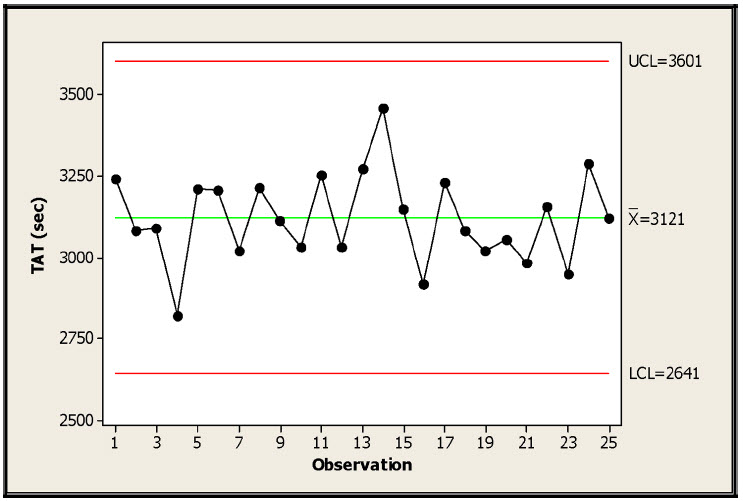
\includegraphics[scale=0.5]{carte.jpg}
        \caption{Exemple de carte de contrôle}
\end{center}
\end{figure}\\
Il existe plusieurs types de graphiques de contrôle, varie par rapport à le type de variable : quantitative, qualitative...\\








\chapter{Six Sigma dans une industrie textile }
\section*{Introduction}
\addcontentsline{toc}{section}{Introduction}
Les marques textiles accordent une attention particulière envers la conformité des mesures dimensionnelles et spécialement à la clientèle. La direction générale de SARTEX a pris la décision de lancer un projet d’amélioration de la qualité qui dure environ 4 mois et elle a exigé le choix de la méthodologie Six Sigma.

Dans le présent chapitre on va présenter les résultats d’étude de cas : mise en œuvre de la méthodologie Six Sigma dans SARTEX.\\
Le travail va être décortiqué par la suite en cinq étapes: les étapes de la méthode DMAIC (développée dans chapitre 3) en consommant les outils appropriés afin d'aboutir à l'objectif désiré.

Les logiciels utilisés dans l'étude : \\
\underline{Minitab} : c’est un logiciel propriétaire commercial de statistiques, qui est utilisé dans les universités pour enseigner les statistiques et aux entreprises qui suivent la méthode Six Sigma.

\begin{center}
    
\includegraphics[scale=0.2]{minitab.png}
\end{center}
\underline{R Studio} : c'est un environnement de développement gratuit et libre pour R, utilisé pour le traitement de données et l’analyse statistique. Dont Shiny est un package R  pour la création d'applications Web interactives directement à partir de R.

\begin{center}

\includegraphics[scale=0.05]{rr.jpg}
\end{center}
\underline{Microsoft Visio} : est un logiciel de diagrammes et de synoptiques (Microsoft Office).
\begin{center}
    
\includegraphics[scale=0.15]{visio.jpg}

\end{center}



\newpage
\section{Phase DEFINIR}
Dans cette phase il faut y répondre à ces questions clés : 
Quels sont les objectifs ?
Quelle échéance ?
Qui fait quoi ?
Quels sont les résultats attendus ?\\
D’autre part il faut clarifier et dessiner une carte du processus détaillée à étudier.

\subsection{Charte de projet}
Donc comme une point de départ, dans un cadre formel, il faut élaborer un document qui donne l'autorité au sponsor et chef d'équipe pour allouer l'équipe qui va travailler dans ce projet. Ce document, c'est la charte du projet qui résume l'objectif, l'équipe, le planning...

\begin{figure}[!h]
\begin{center}
        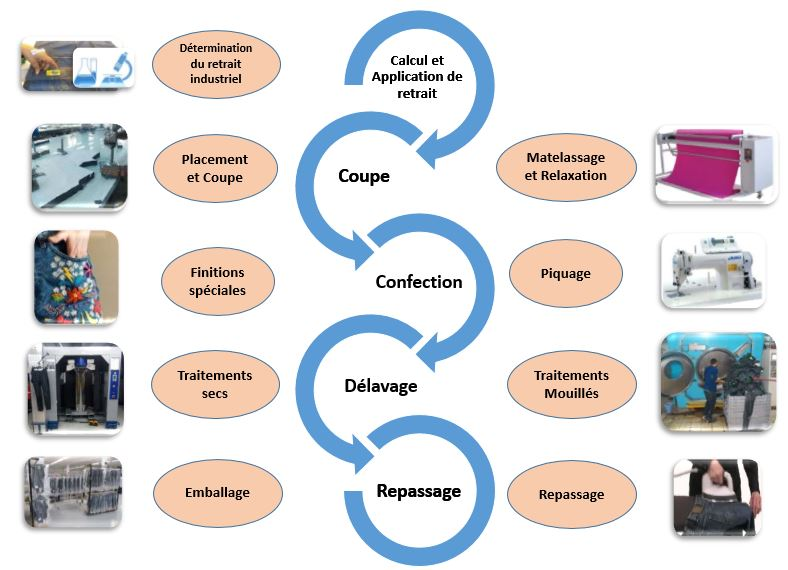
\includegraphics[scale=0.75]{facteur.JPG}
        \caption{Processus général}
\end{center}
\end{figure}
\paragraph*{\textbf{Objectif du projet} :} dans ce projet, on va s'intéresser à la phase développement : prototype Collection et Size Set seulement sur l'article pantalon. Le produit passe par plusieurs phases de production (Fig. 4.1) et subit plusieurs actions ce qui donne naissance à la variation et la variabilité de processus et par conséquent des réclamations client. Donc l'objectif du projet est de réduire cette variabilité, les réclamations, les pénalités, les retouches internes, etc. Et donc améliorer la qualité globale par la réduction de non-conformité.
\paragraph*{\textbf{L'équipe} :} la réussite du projet est liée à une équipe compétente, motivée et impliquée. Le choix de membres s'est fait par le chef d’équipe et le sponsor que doit être réfléchi d'une façon que l'équipe soit hétérogène, constitué de différents départements et de différentes spécialités.\\
En raison de la confidentialité des informations concernant les membres, ils vont être mentionnés par leur fonction :\\
- Champion : directeur général de SARTEX.\\
- Sponsor : directeur qualité. \\
- Chef d'équipe : chef produit.\\
- Les membres : 15 personnes de diverses fonctions.


\paragraph*{\textbf{Le planning} :} le projet dure environ 4 mois ou plus, avant d'y commencer, il faut repartir approximativement cette durée en 5 parties (selon DMAIC). Le but, c'est de clarifier le schéma à suivre et toute l'équipe se met d'accord (voir annexe \ref{nour}
)


L'élaboration de charte du projet nécessite finalement la validation de membres spécialement le contrôleur de gestion, le sponsor et le champion.
Ce document est dynamique qui pourra être modifié tout allons le projet dont l’identification des indicateurs de performance que seront fixés ultérieurement, on élaborant la voix du client et par la suite fixer des objectifs SMART.
\begin{center}
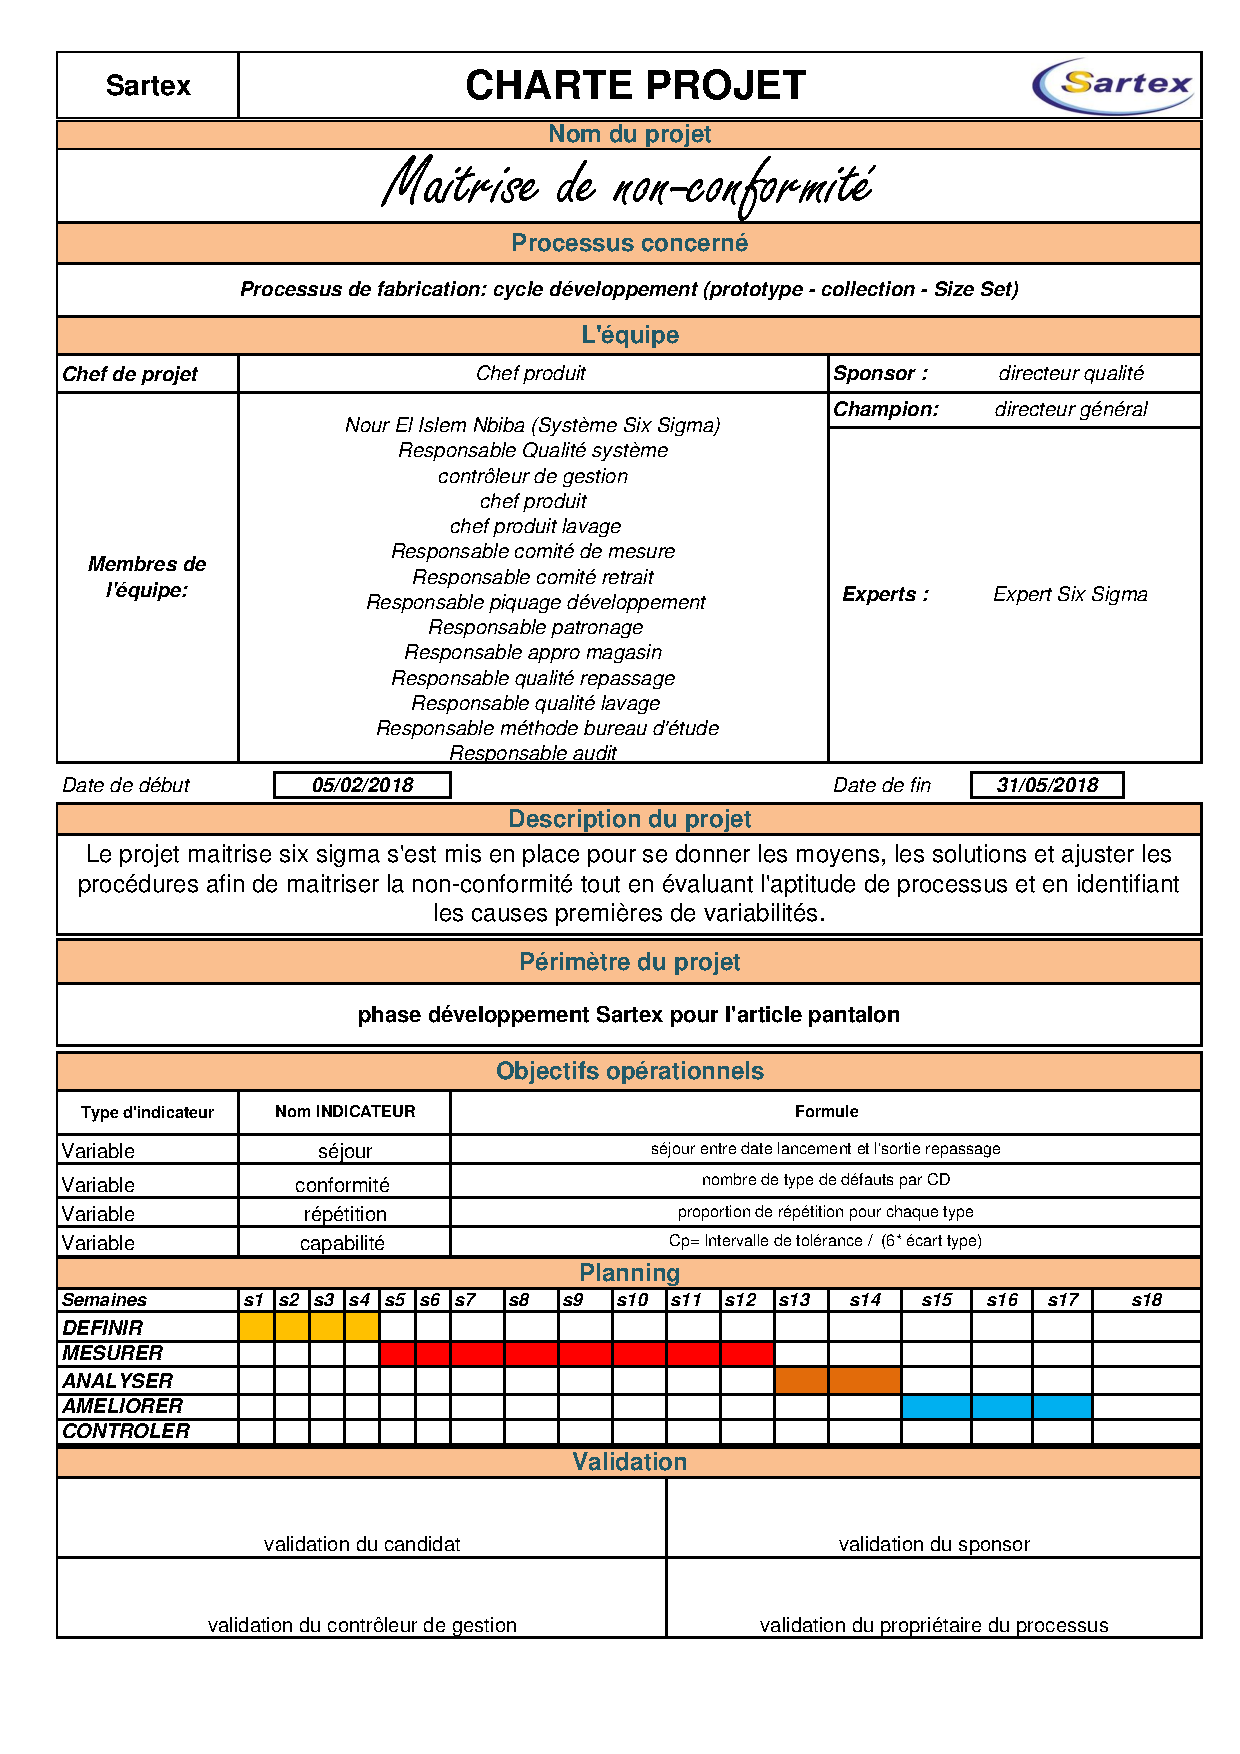
\includepdf[pages=1]{pfee.pdf}
 \end{center}
\begin{table}[!htbp]
\begin{center}
\caption{Charte de projet}
 \end{center}
\end{table}
\subsection{Flux de processus}
Le flux de processus chez SARTEX est trop compliqué dont l'existance de plusieurs unités de fabrication.
Selon l'étape de la phase développement et le demandé client, le schéma suivi diffère donc il est indispensable d'avoir une vue globale et claire du processus pour chaque étape.
\begin{center}
        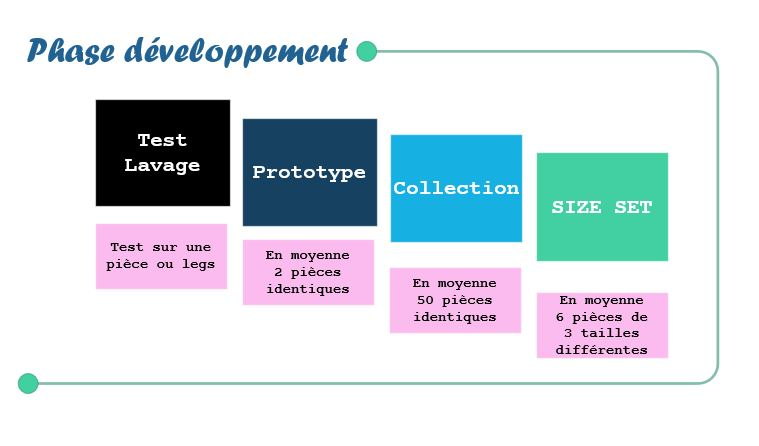
\includegraphics[scale=0.7]{phases.JPG}
\end{center}

L'objectif de schématisation de processus pour le projet \textbf{Maîtrise de non-conformité}:
\item - La compréhension du flux de processus.
\item - Facilite l'identification de source variabilité et la localisation des problèmes.
\item - Connaître le plan de contrôle. 
\item - Connaître les inputs et les outputs.
\item - Permettre l'équipe de voir les choses de la même façon et se mettre d'accord sur un flux commun.


L'idée était de schématiser le flux sans s'appuyer sur aucune documentation fournie par l'entreprise. Le but est de visualiser le flux \underline{existant} non pas le censée être suivie et  être au courant de la situation réelle actuelle.\\
\paragraph*{Démarche:}
\item 1- Recueillir des informations en détails de tous les départements concernant chaque étape (test lavage, prototype, collection et Size Set).
\item 2- Élaborer un schéma du flux de processus (copie zéro).
\item 3- Valider les schémas avec les personnes concernés (faire des modifications si nécessaire).
\item 4- Se réunir et discuter les schémas avec équipe Six Sigma et les personnes concernées, et vérifier s'il existe des incohérences entre les informations ou des malentendus.
\item 5- Valider les schémas par toute l'équipe et les personnes concernées.\\
Ces étapes résultent quatre synoptiques détaillés (\textbf{voir annexe \ref{nour11} }) 
\begin{figure}[!h]
\begin{center}
     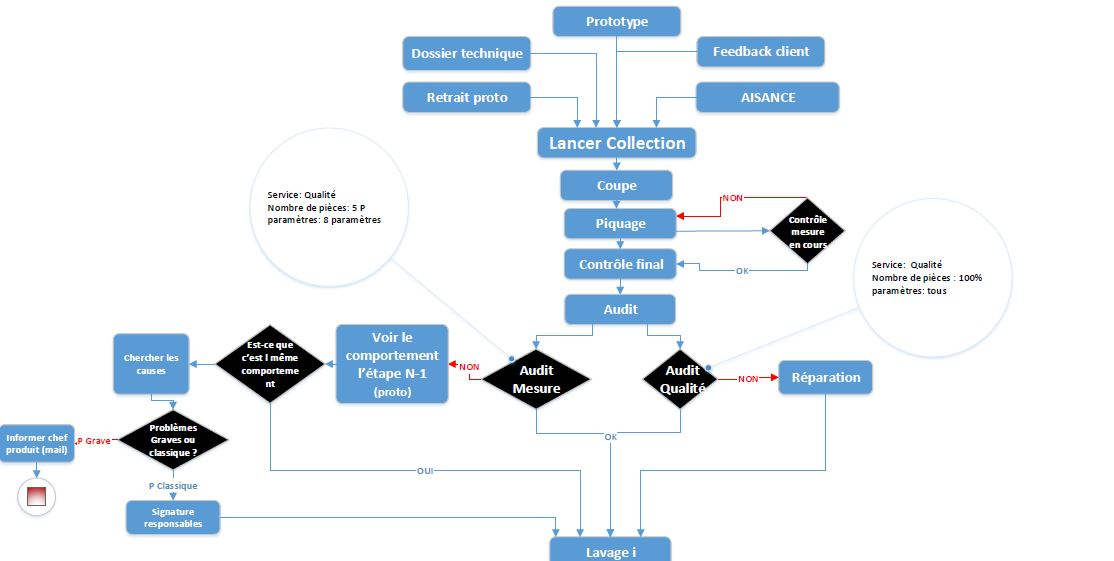
\includegraphics[scale=0.65]{coll.JPG}
     
        \caption{Extrait du synoptique du flux de processus (collection) }
\end{center}
\end{figure}

















\subsection{Voix du Client VOC}

Le départ d'élaboration de VOC est basé sur les feedbacks client, exigences clients et ses attentes. Le point de mire de VOC est pour aboutir à des indicateurs de performance appropriés et calculables.\\
C'est pourquoi on a procédé comme suit (figure 4.3) :
\begin{figure}[!h]
\begin{center}
     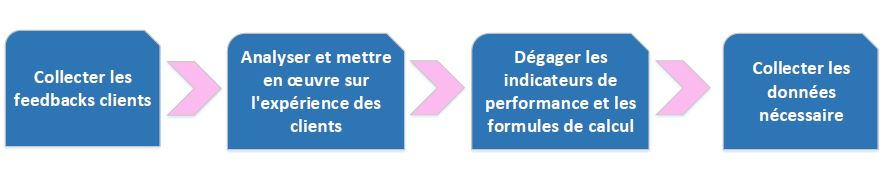
\includegraphics[scale=0.7]{vo.JPG}
     \caption{Etapes d'élaboration de VOC}
\end{center}
\end{figure}\\

Suite à des réunions successives avec l'équipe du projet Six Sigma Maitrise de non-conformité, on a dégagé les indicateurs suivants qui sont la synthèse des données clés de l’entreprise SARTEX :
\item \textbf{Séjour} : c’est le délai de séjour d’un CD.
\item \textbf{Conformité} : c’est nombre de type de défauts par CD 
\item \textbf{Répétition} : c'est la proportion qu'un CD se relance au moins une fois.
\item \textbf{Capabilité} : c’est la capabilité de processus de production.\\

Subséquemment, on a défini les formules de calcul. Le problème se pose étais la validation finale des formules, car tout dépend de données fiables et existantes.\\
La situation nécessite donc une étude complète d’existant, développée par la suite, pour chaque indicateur afin de : 
\item - Bien défini chaque indicateur.
\item - Valider les formules de calcul et calculer les indicateurs.
\item - Connaître les données disponibles.
\item - Détecter les modes de défaillances et les lacunes existantes.\\

On peut enfin récapituler ce VOC dans dans tableau (voir tab 4.2).
\begin{center}
     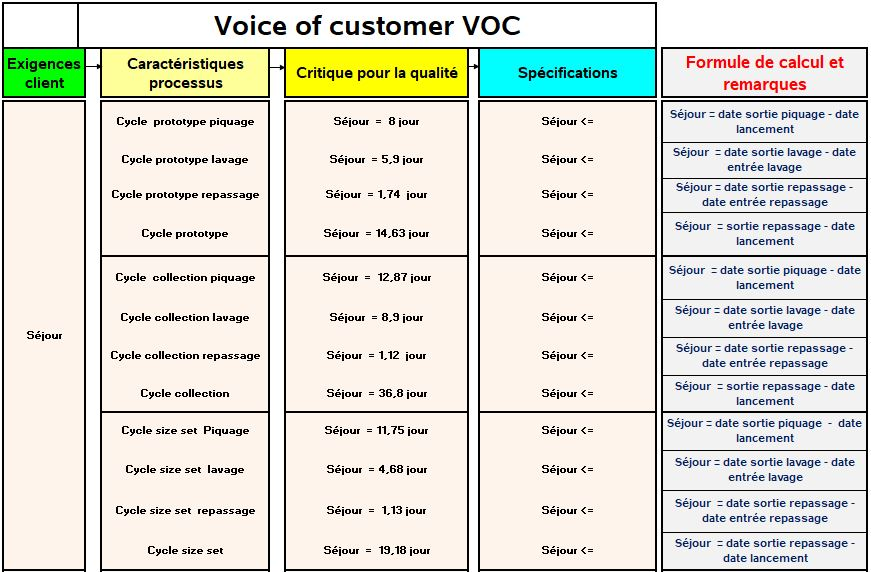
\includegraphics[scale=0.7]{1.JPG}
 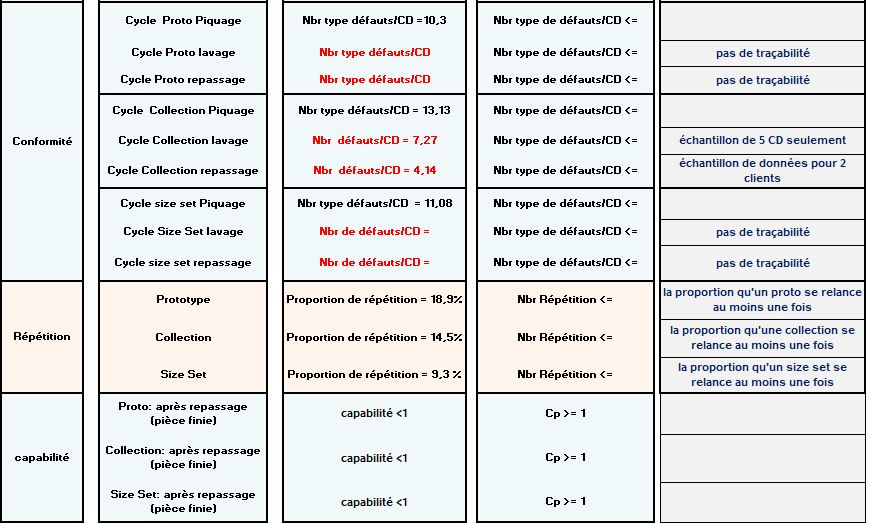
\includegraphics[scale=0.7]{2.JPG}
\end{center}
\begin{table}[!htbp]
\begin{center}
\caption{Voice Of Customer VOC}
 \end{center}
\end{table}

 \subsection{Etude préliminaire d'indicateur Séjour}
Pour bien englober l'indicateur séjour pour chaque étape (prototype, collection et Size set) , il faut :
\item - Décortiquer les phases du séjour par étape de production.
\item - Schématiser les étapes pour avoir une vue claire et globale.
\item - Connaître les dates disponibles et les non-disponibles. 
\item - Connaître les bases dans lesquelles les départements enregistrent les dates.

La schématisation suivante représente le flux du séjour et la différence entre le séjour qu'on peut le calculer, séjour réel, et le séjour idéal qu'on veut calculer.\\
\textbf{Les problèmes:}
\item - Non-traçabilité de données dans plusieurs départements (ce sont les étapes marquées en rouge sur le schéma.)
\item - Les dates enregistrées dans la base développement ne sont pas à jour.
\item - Pour déterminer la date exacte de séjour, les dates doivent être saisies par heures.\\
\textbf{Les formules de calcul du séjour:}
\begin{center}
Séjour = Date Réception client - Date demande client +1       (3)\\  
Séjour piquage = Date Sortie piquage - Date lancement charge +1       (4)\\
Séjour lavage = Date sortie lavage - Date entrée lavage +1        (5)\\
Séjour repassage = Date sortie repassage - Date entrée repassage +1       (6)\end{center}
\begin{center}
 \includepdf[pages=1,angle=90]{sjour.pdf}
 \end{center}
 
 
 
 
\subsubsection{Séjour prototype}

\textbf{Collecte et sélection de données prototypes :}\

Afin de raffiner l'étude, on a éliminé : \

- 24 clients parmi 38 que sont des clients passager ou non potentiel\

- 14\% de charges qui ont des séjours aberrantes entre 31 et 150 jours (fabriquées dans des conditions anormales). \\

- 18,9\% des charges version 2, 3, 4, 5 et 6, car ils ont une durée de traitement très courte.\\

On obtient donc une base de données contient 1708 prototypes pour 14 clients les plus représentatives durant l'année 2017.\\

 \textbf{Classification des clients selon nombre de charges}\

Dans le dessein de classer les clients selon nombre de charges prototypes, on a construit le diagramme de Pareto (fig 4.4).

 \begin{figure}[!h]

 \begin{center}

 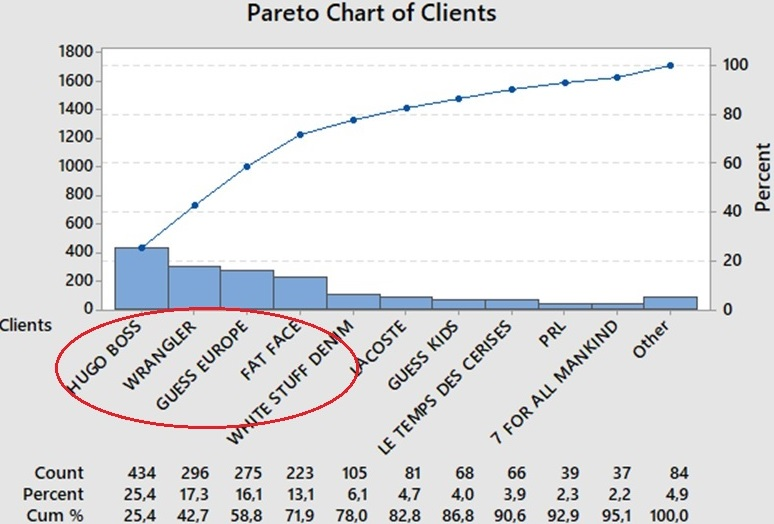
\includegraphics[scale=0.65]{parProto.jpg}

 \caption{Diagramme de Pareto de client selon le nombre de charges }

 \end{center}

\end{figure}

$ \Longrightarrow$ Les clients les plus importants sont 5 clients parmi 14 qui ont  80\% de charges et les plus représentatifs.\\

 \textbf{La répartition du séjour}\\

 \begin{figure}[!h]
 \begin{center}
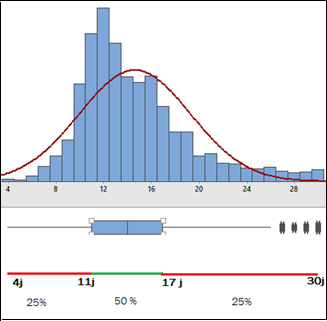
\includegraphics[scale=0.9]{reparproto.png}
 \caption{La répartition du séjour prototype}
 \end{center}
 \end{figure}
 
 
Moyenne séjour = 14.63 jour.\\
Médiane = 14 jour. \\
50\% de prototypes ont des séjour entre [11 ,17] jour.\\
Il y a des valeurs séjour abérrantes proche de 30 jour.\\ 


Afin de savoir si le séjour dépend du client, on a fait un test ANOVA
\begin{center}
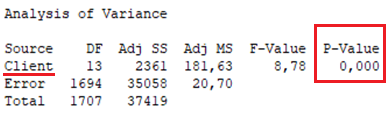
\includegraphics[scale=0.9]{anova.png}
\end{center}

P-Value = 0 < 0.05 $\Longrightarrow$ Le séjour dépend significativement du nom client.\\

Pour visualiser la différence entre les clients, on a figuré leur boxplots.

\begin{center}

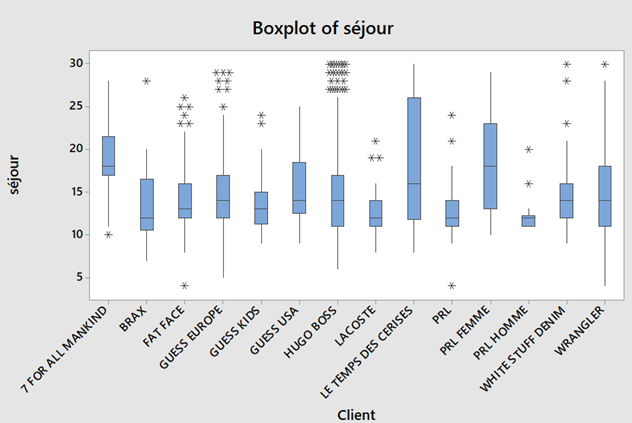
\includegraphics[scale=0.7]{boxproto.png}

\end{center}

$\Longrightarrow$ Les boxplots montrent clairement la différence entre les clients.\

En effet, il y a des clients qui ont une grande variabilité de séjour comme : Le Temps Des Cerises, PRL Femme ... et des clients quiont presque la même distribution comme : Hugo Boss et GUESS Europe.








\subsubsection{Séjour colletion}
On refait le même travail  :pour les collections\\
\textbf{Collecte et sélection de données des collections:}\\
Comme première étape on a éliminé :
\item - 8 clients parmi 20 qui sont des clients non-potentiels.
\item - 8\% de charges qui ont des séjours aberrantes supérieur à 60 jours. (fabriquées dans des conditions anormales).
\item - 15.24\% des charges version 2 et 3, car ils ont une durée de traitement très courte.

On obtient donc une base de données contient 832 collections pour 12 clients les plus représentatives durant l'année 2017.\\
\textbf{Classification des clients selon nombre de charges}\\
Idem, on a construit le diagramme de Pareto (fig 4.15) pour classer les clients.\\
\begin{figure}[!h]
\begin{center}
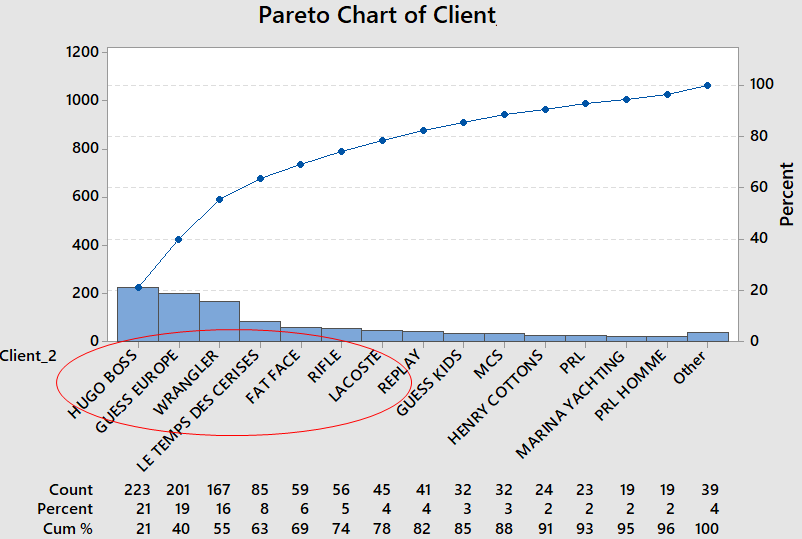
\includegraphics[scale=0.65]{parcoll.png}
\caption{Diagramme de pareto de client selon les charges collections}
\end{center}
\end{figure}\\
$\Longrightarrow$ Les clients les plus importants sont 8 clients parmi 12 qui ont 80\% de charges et les plus représentatifs.\\

\textbf{La répartition du séjour collection}


\begin{figure}[!h]
\begin{center}
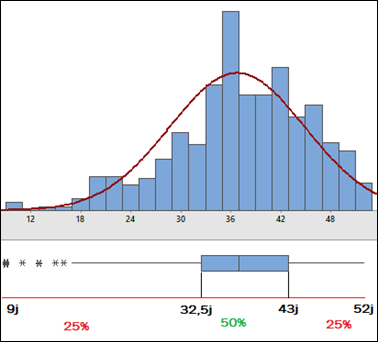
\includegraphics[scale=0.85]{reparcoll.png}
\caption{La répartition du séjour collection}
\end{center}
\end{figure}
Moyenne séjour = 36.8 jour.\\
Médiane = 37 jour. \\
50\% de prototypes ont des séjour entre [32.5 , 43] jour.\\
Il y a des valeurs séjour abérrantes proche de 9 jour.\\ 
La quantité moyenne de piéces es égale à 41.01 qui varie entre [2 , 122].\\





La différence entre les prototypes et les collections que le nombre de pièces de prototype presque fixe (2 pièces) alors que pour la collection varie dans l'intervalle [2 , 122], donc il est important d'étudier la corrélation entre le séjour et la quantité produite.

\begin{center}
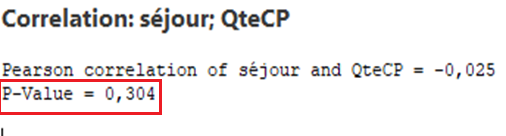
\includegraphics[scale=0.8]{corr.png}
\end{center}
P-Value = 0.304 > 0.05 $\Longrightarrow$ non significative.\\
Ici, on peut affirmer qu'il n'existe pas une corrélation entre la qualité et le séjour.\\
 
 
Les boxplots ci-dessous permettant de visualiser la différence entre les clients et de montrer clairement la grande différence entre les clients.
\begin{center}
\end{center}


\begin{figure}[!h]
\begin{center}
     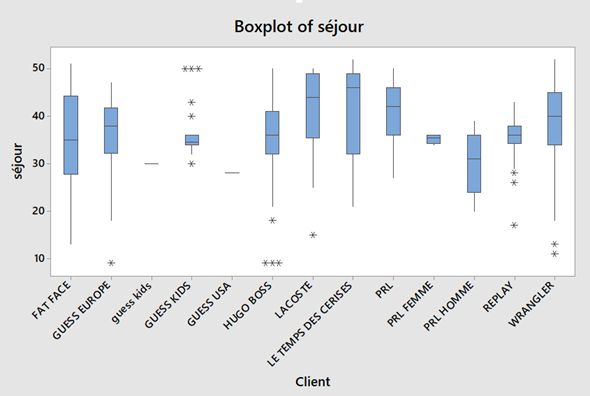
\includegraphics[scale=0.8]{boxcoll.png}
\caption{Les boxplots du séjour collection par client}
\end{center}
\end{figure}

On peut voir que les boites sont de tailles différentes et de moyennes différentes




\subsubsection{Séjour Size Set}
\textbf{Collecte et sélection de données des Size Set:}\\
Comme première étape on a éliminé :
\item - 11 clients parmi 25 qui sont des clients non-potentiels.
\item – 9.3\% des charges version 2 et 3, car ils ont une durée de traitement très courte.
La base de données qu’on va travailler avec contient 946 Size Set pour 14 clients pour l’année 2017.\\


\textbf{Classification des clients selon nombre de charges}\\

Idem, on a construit le diagramme de Pareto (fig 4.15) pour classer les clients.\\
\begin{figure}[!h]
\begin{center}
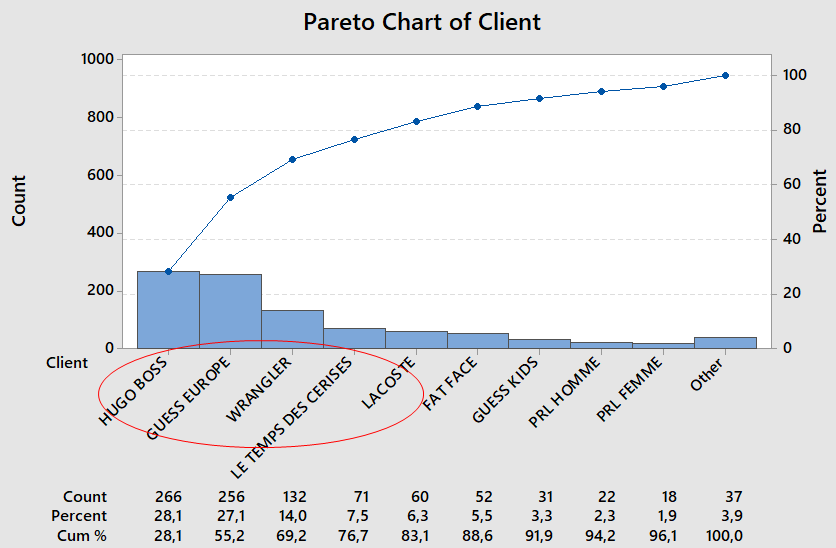
\includegraphics[scale=0.7]{parsize.png}
\caption{Diagramme de pareto de client selon les charges size set}
\end{center}
\end{figure}\\
$\Longrightarrow$ Les clients les plus importants sont 5 clients parmi 14 qui ont 80\% de charges et les plus représentatifs.\\


\textbf{La répartition du séjour Size Set}\\
Moyenne séjour = 19.18 jour.\\
Médiane = 18 jour. \\
50\% de prototypes ont des séjour entre [15 , 22] jour.\\
Il y a des valeurs du séjour abérrantes entre 32 et 42 jour.\\ 


\begin{figure}[!h]
\begin{center}
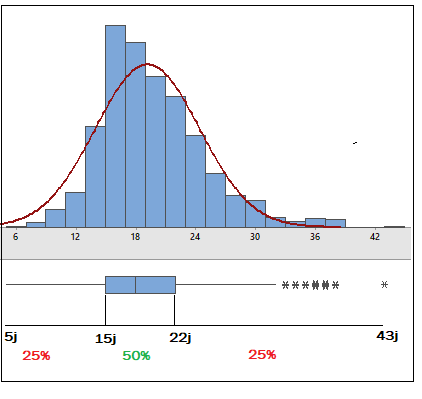
\includegraphics[scale=0.7]{reparsize.png}
\caption{La répartition du séjour Size Set}
\end{center}
\end{figure}

Les boxplots ci-dessous permettant de visualiser la différence entre les clients et de montrer clairement la grande variabilité de séjour entre les clients.
\begin{center}
\end{center}
\begin{figure}[!h]
\begin{center}
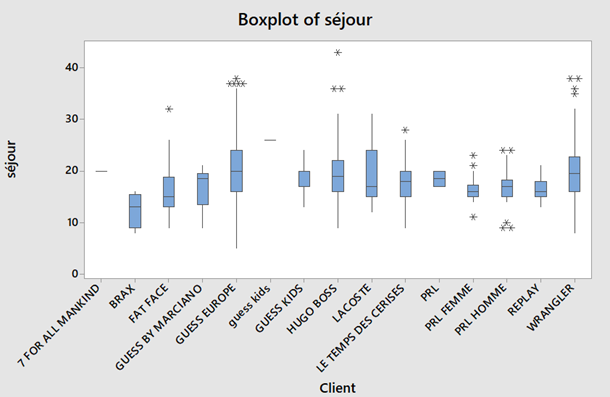
\includegraphics[scale=0.8]{boxsize.png}
\caption{Les boxplots du séjour Size Set par client}
\end{center}
\end{figure}

On peut voir que leur boites sont de taille différentes et de moyennes différentes par contre ils sont plus homogènes que les séjours de collections et size set.







\subsection{Etude préliminaire d'indicateur Conformité}
Pour examiner la conformité, la pièce passe par plusieurs contrôles au cours du cycle de production.
Il existe deux catégories de contrôle de la conformité : 
\item - \underline{Mesure dimensionnelle} par rapport la demande client.
\item - \underline{Visuelle} par rapport la demande client (les défauts, nuance, non-conformité...).\\
Donc il est inévitable d'élaborer un plan de surveillance très bien détaillé des contrôles qui mettent l'accent sur :\\
- La méthode de contrôle : technique, type, référence... \\
- L'échantillonnage : paramètre contrôlé et la taille de l'échantillon\\
- L'enregistrement des données...\\

Et suite à une collecte des informations concernant tous les contrôles, on a pu élaborer ce plan de surveillance bien développé voir Annexe \ref{nour111} .\\
Vu le volume important des informations dans ce document , il était préférable de schématiser ce plan pour facilité la consultation d'information.

\begin{center}
 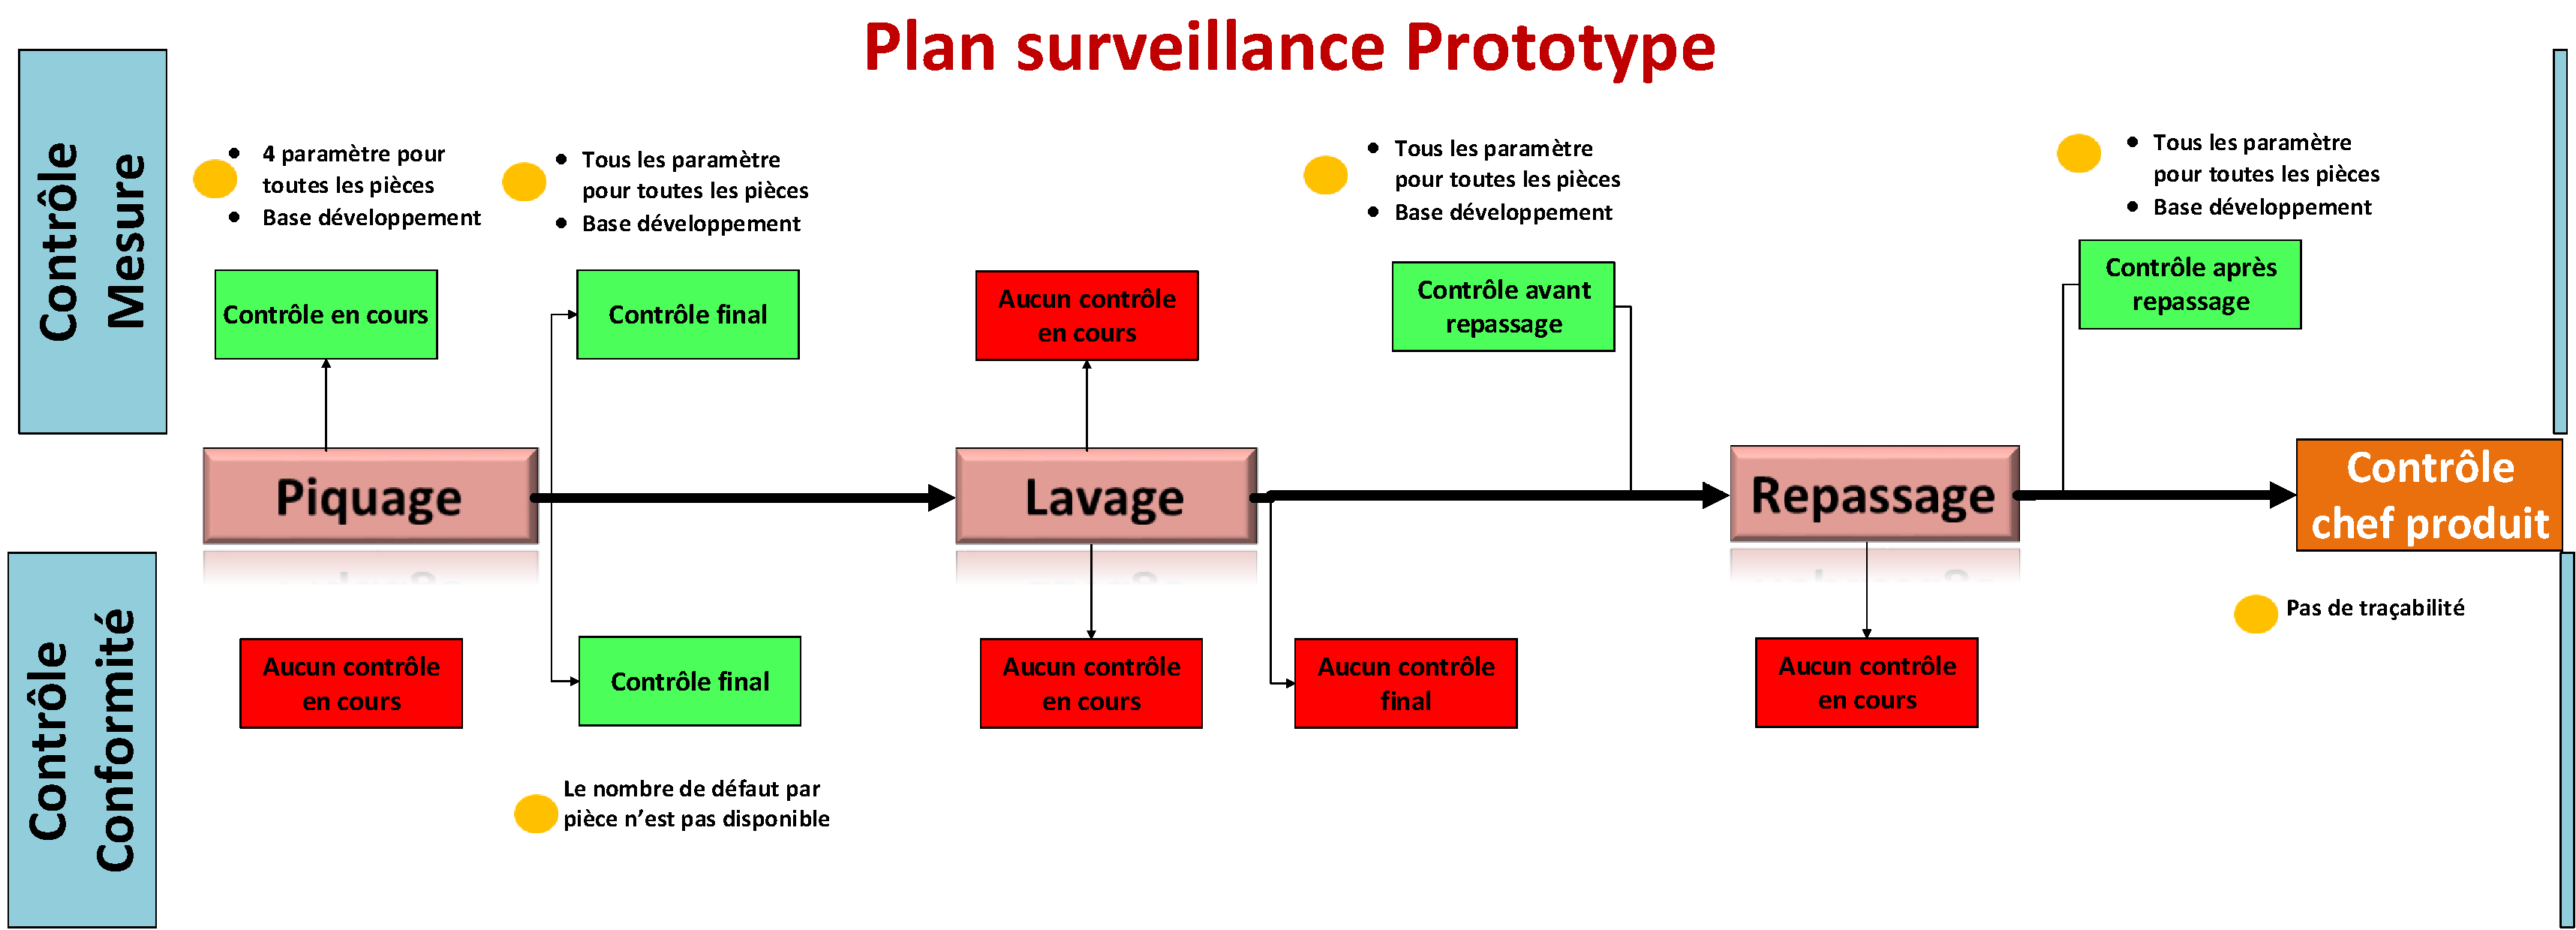
\includepdf[pages=1, angle=90]{contaaa.pdf}\\
  \includepdf[pages=2, angle=90]{contaaa.pdf}\\
 \includepdf[pages=3, angle=90]{contaaa.pdf}

 \end{center}






\section{Phase MESURER}
Après la définition des éléments fondamentaux du projet Six Sigma, on passe à la phase mesurer : la phase de collecte de données.
\subsection{Mesure de performance de système de mesure}
Avant de collecter les données, il est nécessaire de mesurer la performance de système de mesure, cette étape a une importance primordiale.\\
Les tests gage R\&R permettent de qualifier le système de mesure.

On a procédé comme suit :\\
\textbf{\underline{Effectif} :}
\item - Service piquage : 7 agents.
\item - Service lavage : 2 agents.
\item - Service repassage : 2 agents.
\item - Sous-traitance : 14 agents.\\
Les agents sont regroupés en sous-groupes de deux ou trois agents par test.\\
\textbf{\underline{Répétition} :} chaque agent va refaire la prise de mesures 3 fois.\\
\textbf{\underline{Pièces} :} on a sélectionné 10 pièces aléatoirement de différent taille.\\
\textbf{\underline{Paramètres} :} on a fixé 3 paramètres, appelé les grands paramètres (fig 4.10) , ce sont les plus importantes et critiques : tour de taille (AB) , entre jambe (CD) et fond dos (AC).\\
\begin{figure}[!h]
\begin{center}
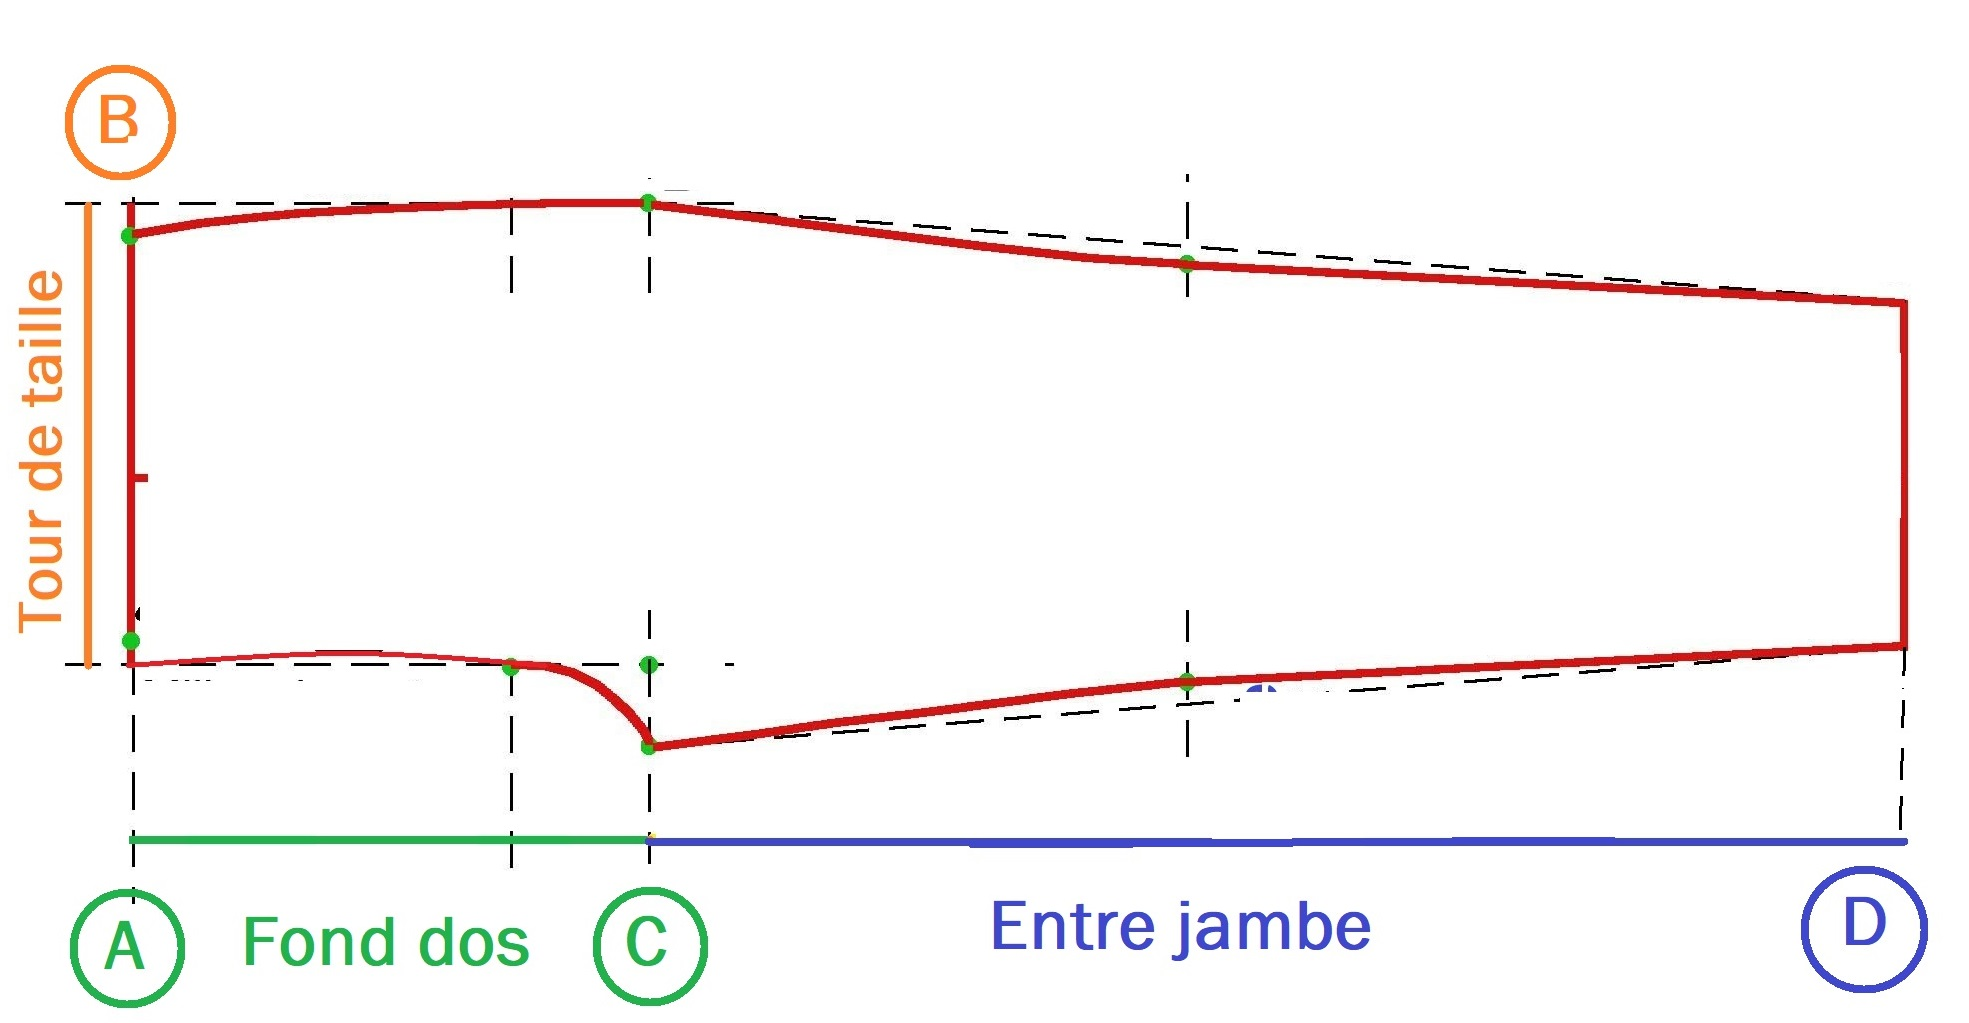
\includegraphics[scale=0.2]{pantalon.jpg}
\caption{Les paramètes à mesurer}
\end{center}
\end{figure}\\

\textbf{\underline{Procédure du test} :} 
\item \textbf{1}- Numéroter les pièces 1 à 10 (les numéros doivent être caché)
\item \textbf{2}- Regrouper les agents de chaque service en groupes de 2 ou 3.
\item \textbf{3}- Créer des feuilles de travail d'étude gage R\&R selon le nombre d'agents (2 ou 3) à l'aide du logiciel \textbf{Minintab}.
\item \textbf{4}- S'assurer que les conditions du travail sont normales et sensibiliser les agents que c'est un test pour évaluer le processus et non pas les agents de mesure. 
.
\item \textbf{5}- Prise de mesures de 10 pièces par chaque agent à part en respectant l'ordre de feuille de relevé.
\item \textbf{6}- Refaire la prise de mesures encore deux fois.
\item \textbf{7}- Traitement de données sur Minitab et analyse de résultats

\textbf{\underline{Analyse de résultats}:}\\
Le but du test est de calculer le pourcentage d'erreur du système de mesures contribuant à l'erreur totale de processus.\\
On a reparti les agents de mesure en 12 groupes, ou chaque groupe fait des tests pour 3 paramètres. Un test dure en moyenne environ 45 minutes pour chaque agent.\\ 
Vu le nombre important d'outputs et le volume de données va étudier un exemple par détail et par la suite récapituler le reste dans un tableau.\\
\begin{figure}[!h]
\begin{center}
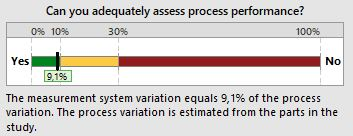
\includegraphics[scale=1]{bgrrtt.JPG}
\caption{Output 1 : test R\&R}
\end{center}
\end{figure}\\
\fbox{\parbox{\textwidth}{ Gage R\&R = 9.14\% \\
$ \Longrightarrow$
La variation du système de mesures représente 9.14\% de la variation totale.\\
$ \Longrightarrow$ 9.14 > 10\% les mesures sont acceptables.\\
}}

\begin{figure}[!h]
\begin{center}
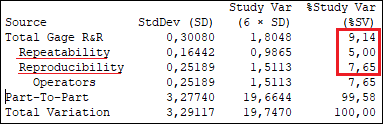
\includegraphics[scale=1]{utrrtt.png}
\caption{Output 2 : test R\&R}
\end{center}
\end{figure}\\

\fbox{\parbox{\textwidth}{ La répétabilité = 5\% \\
$ \Longrightarrow$ C'est la variation résulte lors de la répétition de la même mesure par le même opérateur.\\
$ \Longrightarrow$ Il y a un problème de concentration d'opérateur mais pas du tout grave.}}\\


\fbox{\parbox{\textwidth}{ La reproductibilité = 7.65\% \\
$ \Longrightarrow$ Représente la variabilité entre des opérateurs.\\
$ \Longrightarrow$ Il existe une légère différence entre les méthodes de prise de mesures 
}}

\begin{figure}[!h]
\begin{center}
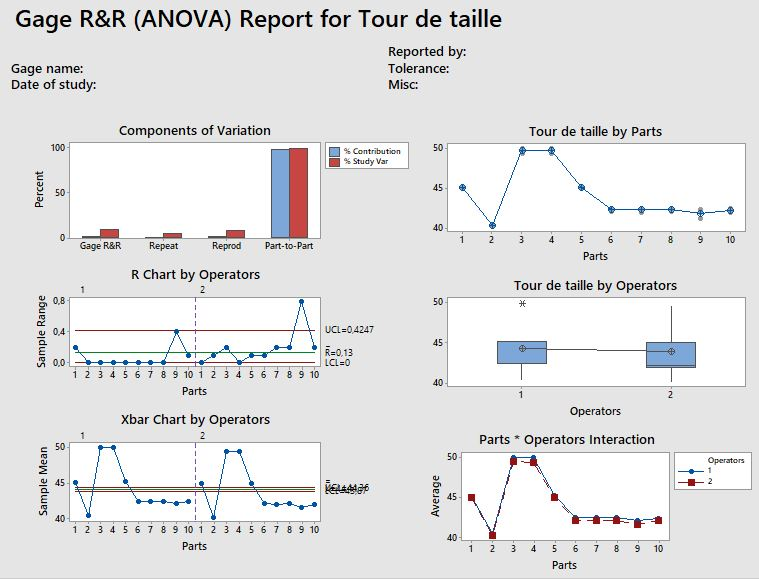
\includegraphics[scale=0.75]{RRTT.JPG}
\caption{Output 3 : test R\&R}
\end{center}
\end{figure}

\fbox{\parbox{\textwidth}{ \textbf{R graphique:} \\
$ \Longrightarrow$ Donne un bon signe, presque toutes les valeurs sont dans l'intervalle de contrôle dont $ \bar{R }= 0.13 $.\\
$ \Longrightarrow$ L'opérateur 2 fait plus de variabilité que l'opérateur 1.\\}}


\fbox{\parbox{\textwidth}{ \textbf{Boxplots :} \\
$ \Longrightarrow$ Les boxplots sont presque identiques. \\
$ \Longrightarrow$ Il n'existe pas une différence remarquable entre les deux opérateurs \\
}} \\




\textbf{\underline{Récapitulation des résultats }:}  voir Tab.4.3\\

\textbf{\underline{Décisons }:}\\


\fbox{\parbox{\textwidth}{ 

Si la répétabilité est élevée \\ $\longrightarrow$ Problème de concentration d'opérateur \\ 
Si la reproductibilité est élevée \\ $\longrightarrow$ Différence entre les méthodes de prise de mesures.\\
$\longrightarrow$Les opérateurs n'ont pas la même formation. 
}}\\


\fbox{\parbox{\textwidth}{ 
Si Gage R\&R < 10\%\\ 
$ \longrightarrow$ Mesure acceptable.\\
$ \longrightarrow$ Refaire un test chaque deux mois.\\
Si 10\% < Gage R\&R < 30\%\\
$ \longrightarrow$ Mesure marginale.\\
$ \longrightarrow$ Refaire le test chaque mois.\\
Si Gage R\&R > 30\% \\
$ \longrightarrow$ Mesure inacceptable (données non-fiables).\\ 
$\longrightarrow$ Reformation des opérateurs.\\
}}





\fbox{\parbox{\textwidth}{ 
\\
Pour poursuivre l'évaluation de performance du
système de mesures après le projet Six Sigma, on a élaboré un manuel de travail du test de mesure R\&R bien détaillé. voir Annexe \ref{nour1111}  \\
}}\\



Donc, suite aux résultats du test, on a planifié une réunion avec tous les agents de mesure (phase développement) pour :

- Présenter et expliquer les résultats.

- Sensibiliser les agents à l'importance de ce genre du test pour eux.

- Sensibiliser les agents de l'intérêt de leur travail pour l'entreprise et que la production est basée sur leurs mesures.\\



\begin{figure}[!h]
\begin{center}
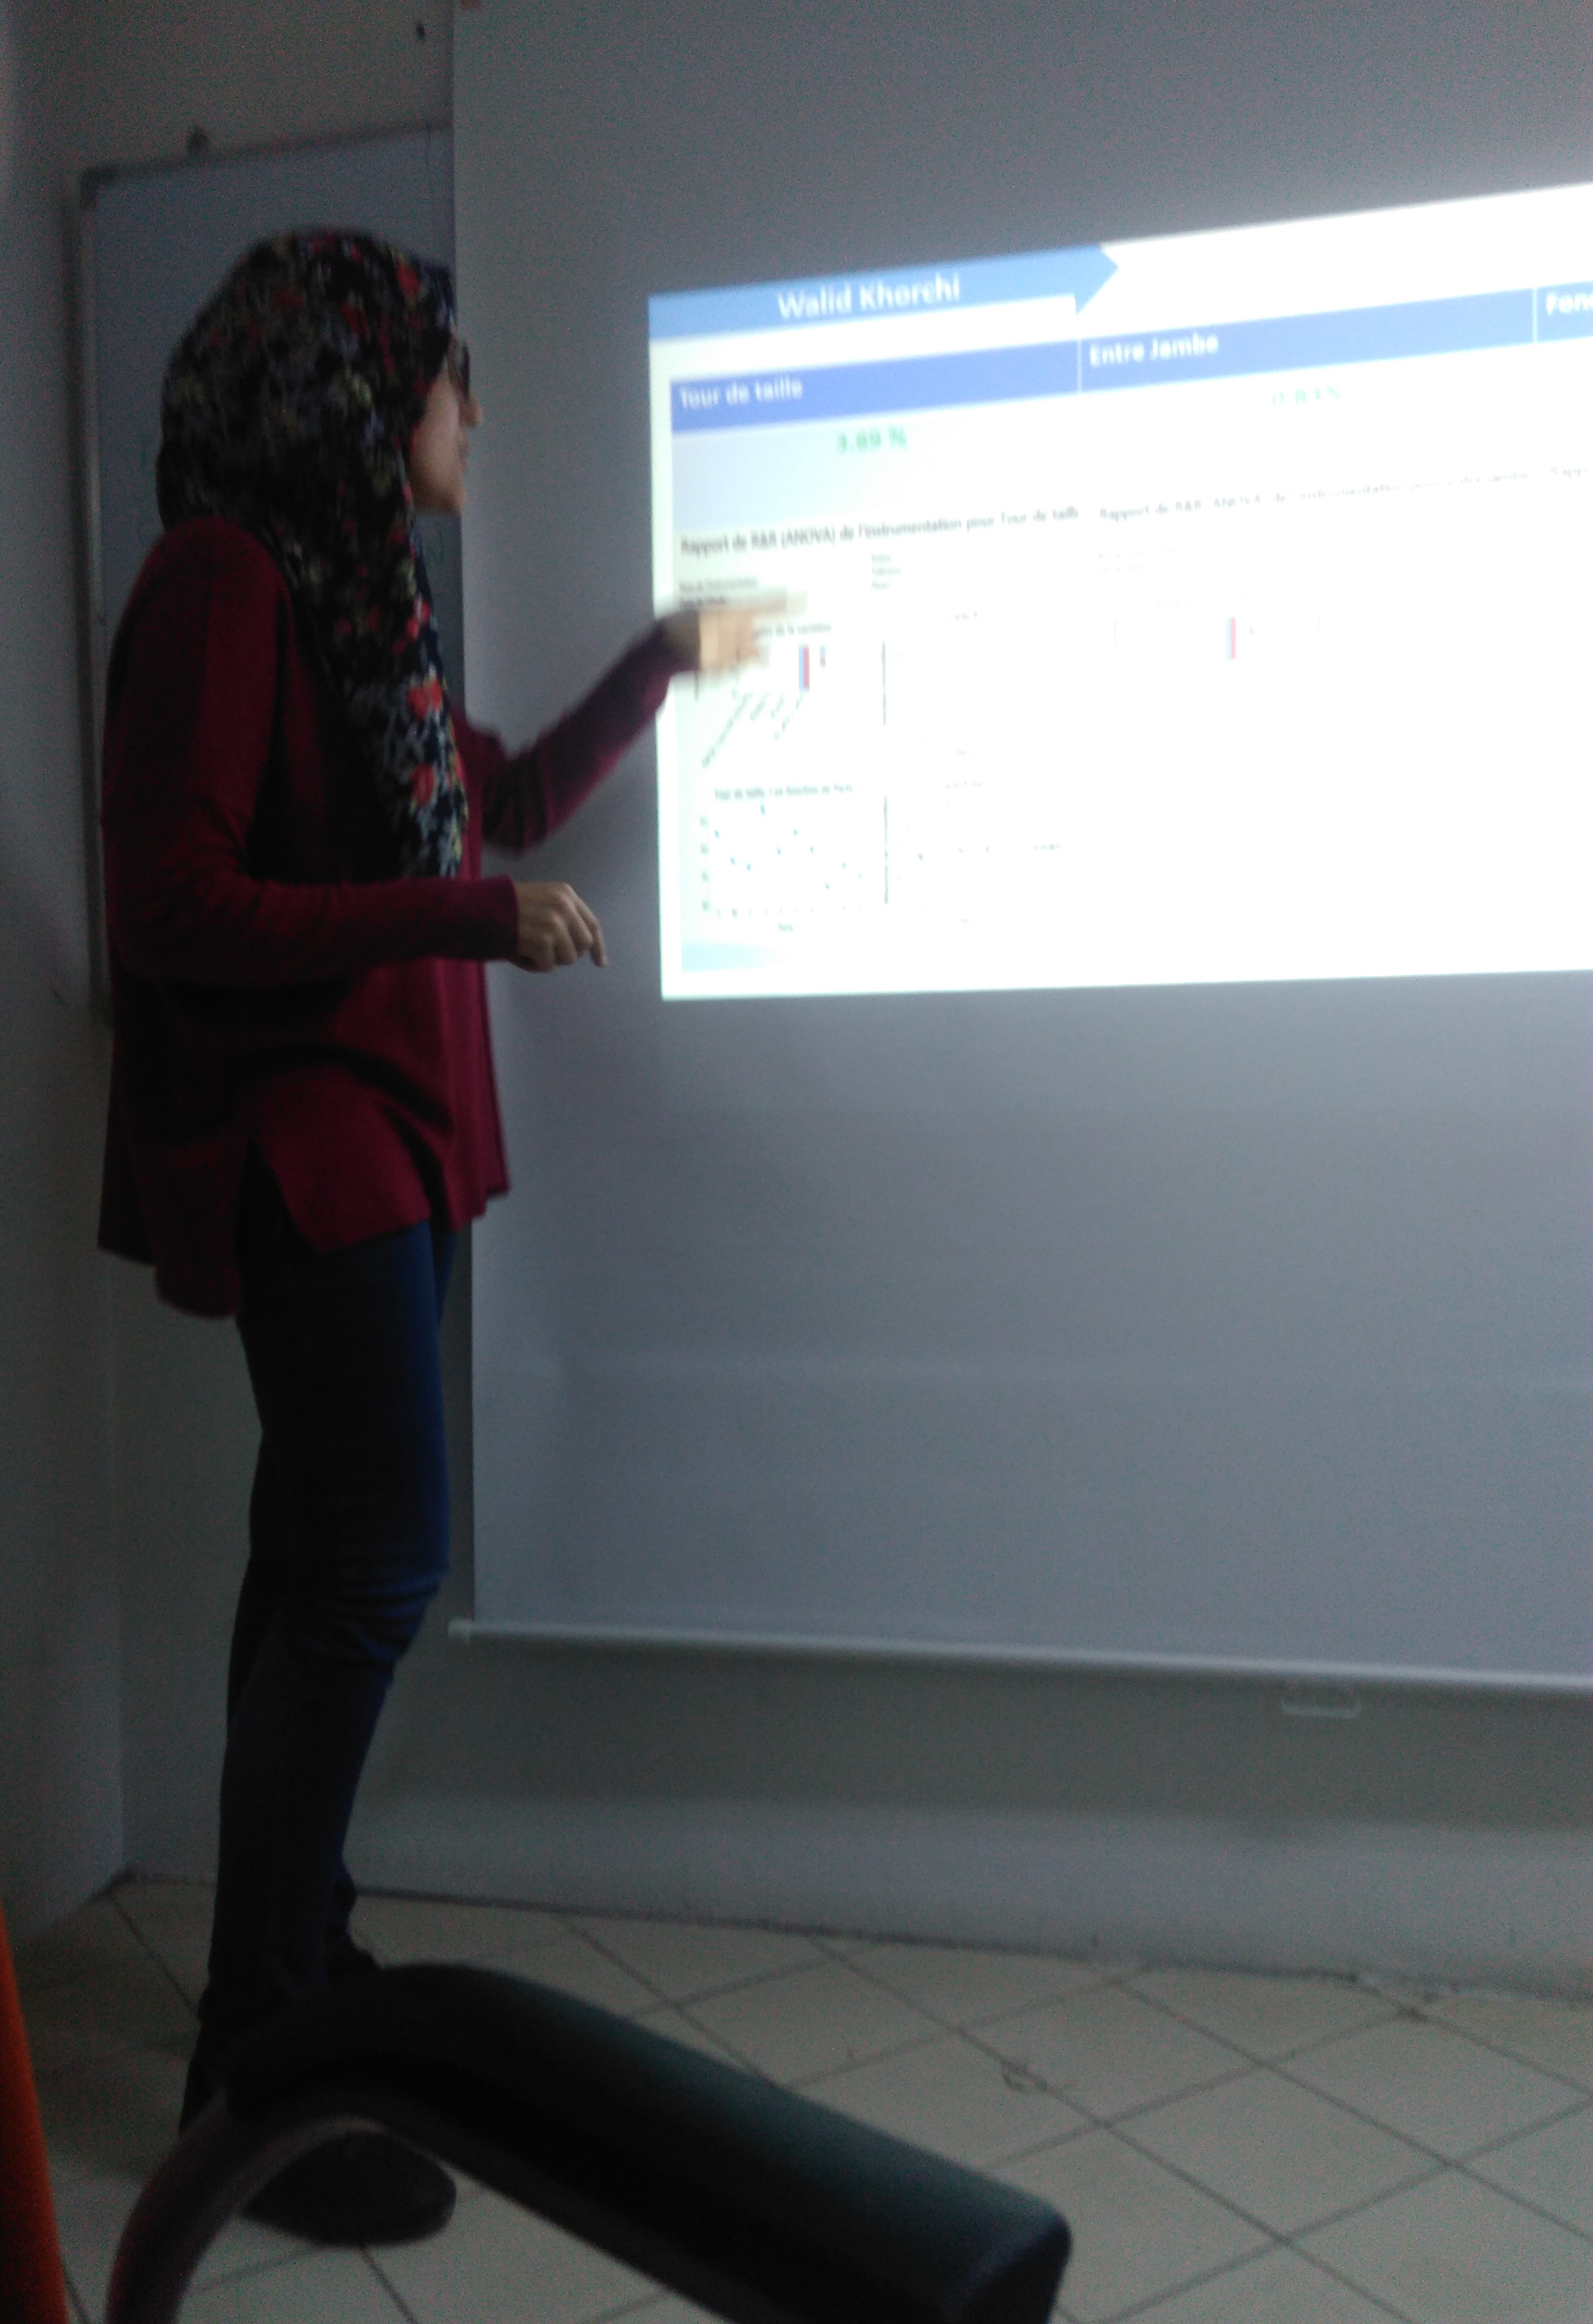
\includegraphics[scale=0.05]{moi.jpg}
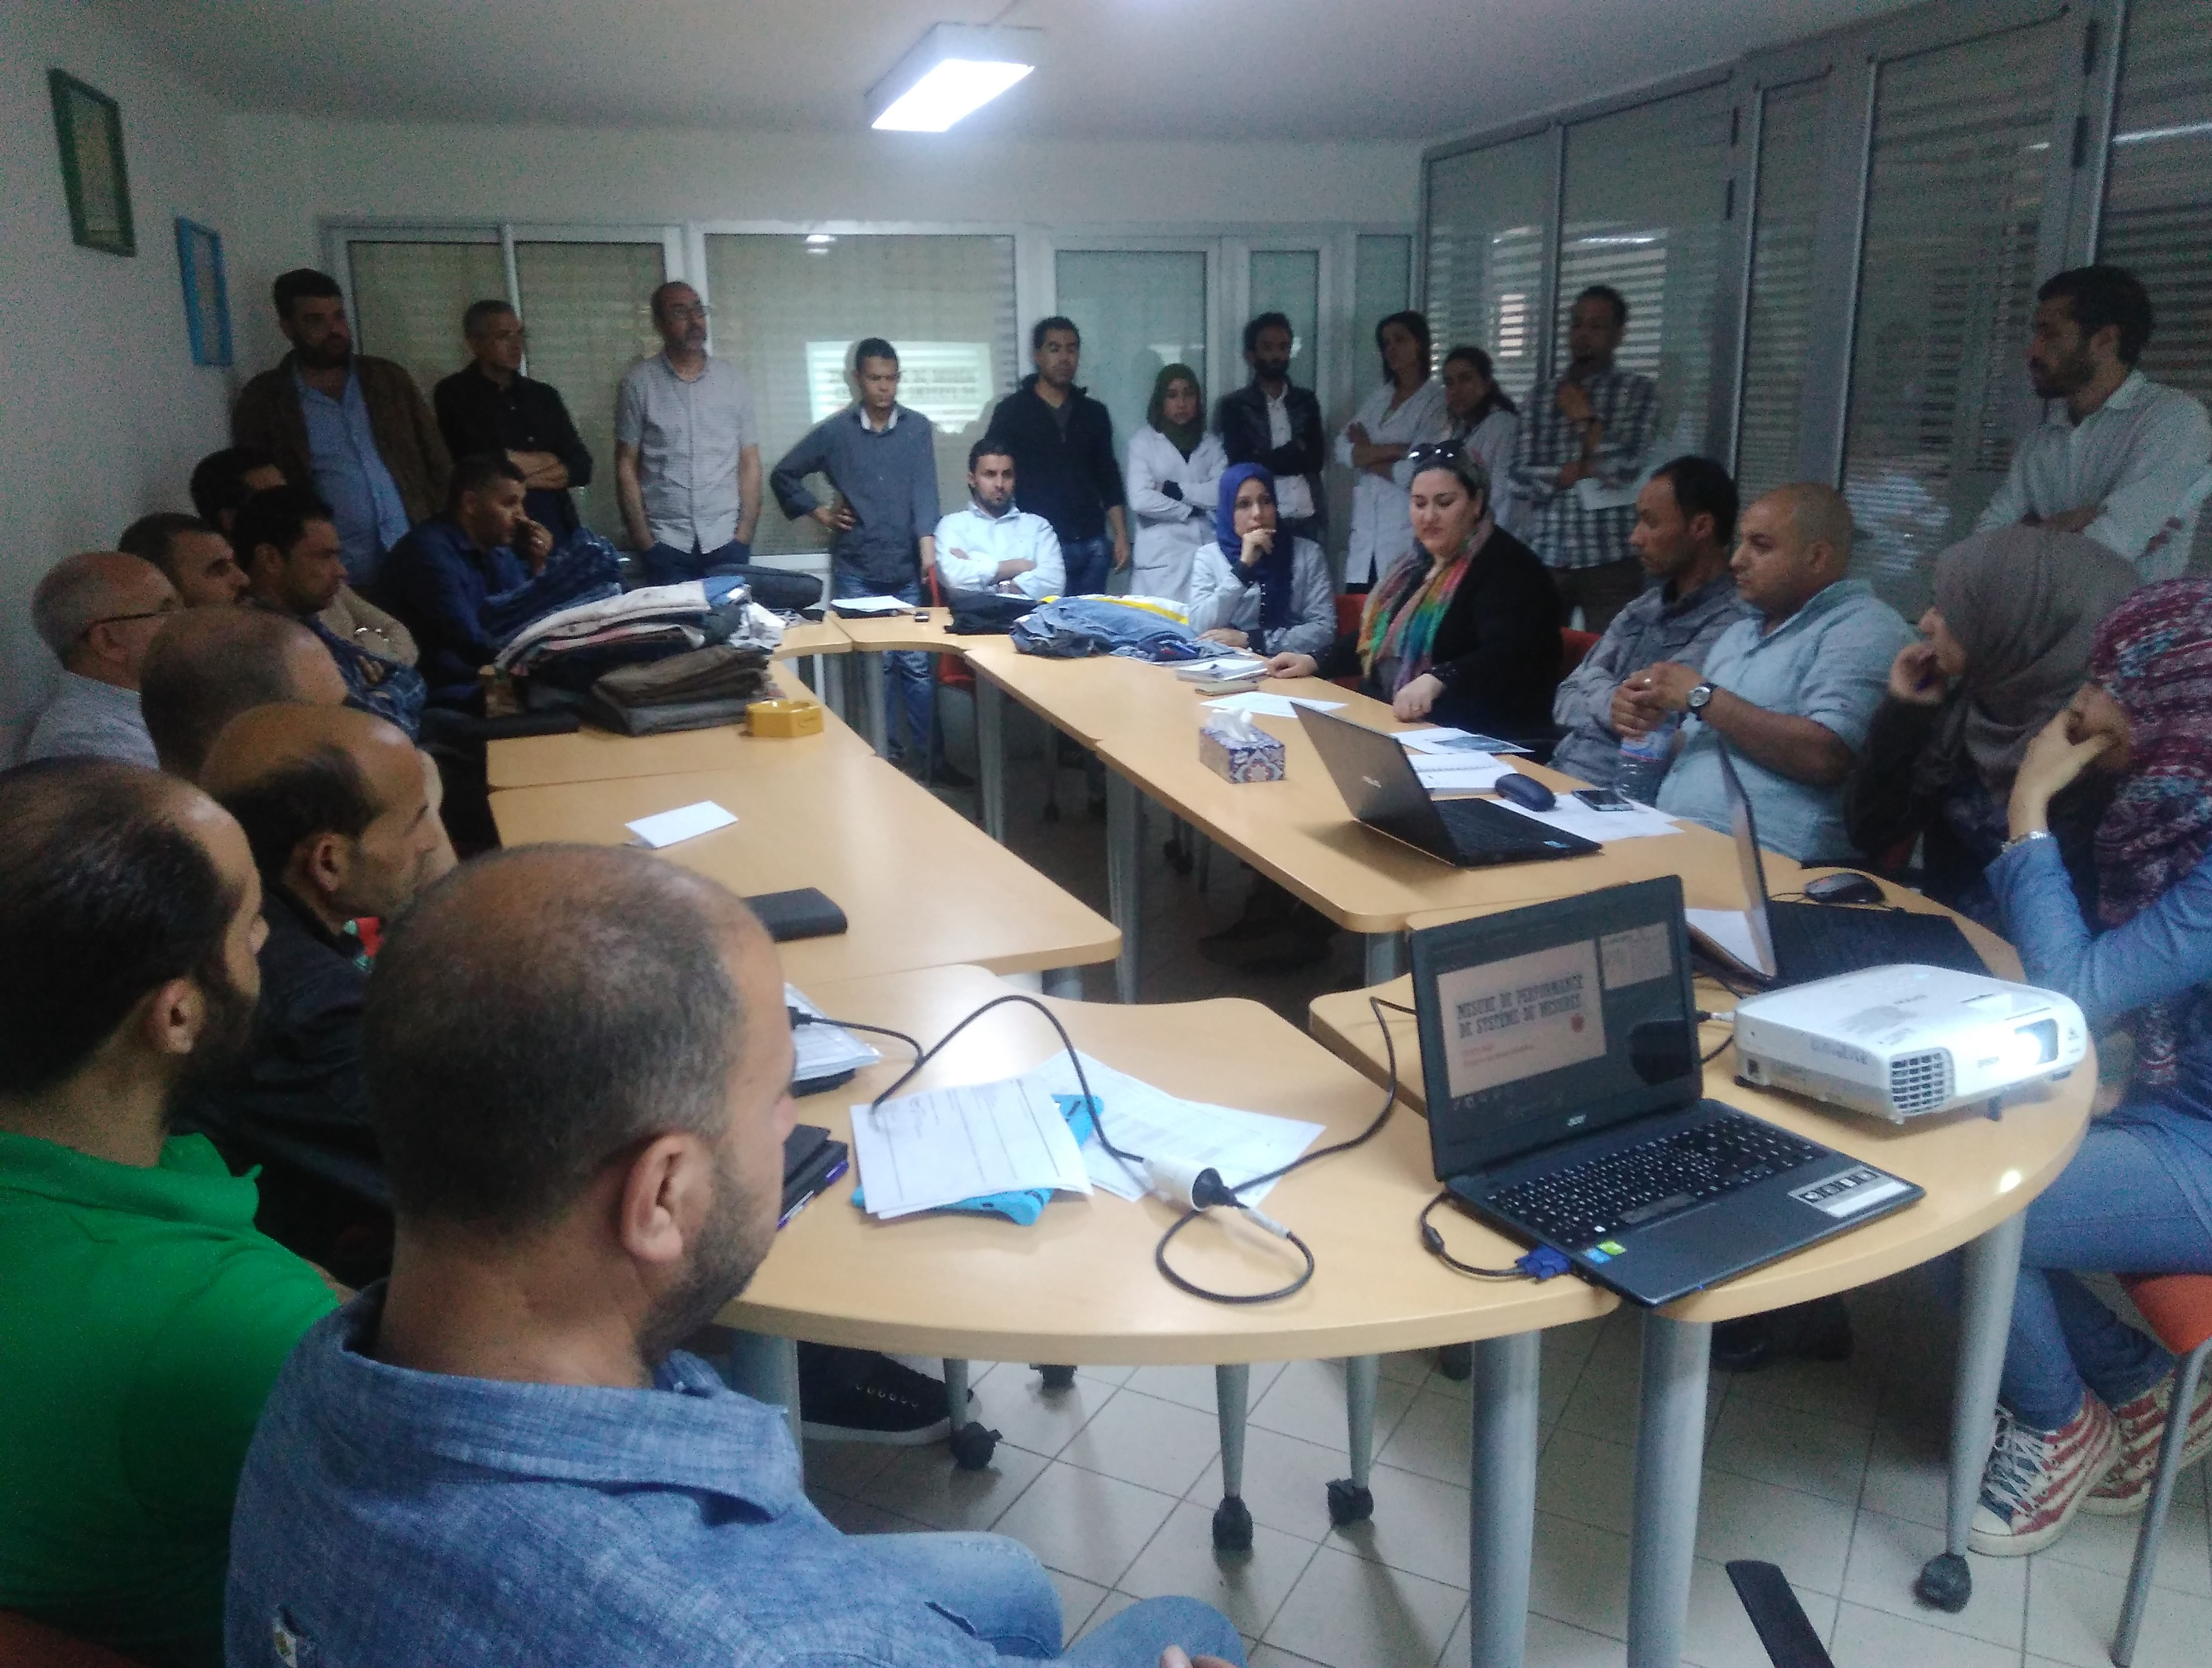
\includegraphics[scale=0.06]{euxbl7a9.jpg}
\caption{Réunion de sensibilisation du test R\&R}
\end{center}
\end{figure}
\begin{table}[!htbp]
\begin{center}
\baselineskip 20pt
\begin{tabular}{|C{2.6cm}|C{0.4cm}||C{1cm}|C{1cm}|C{1cm}||C{1cm}|C{1cm}|C{1cm}||
C{1cm}|C{1cm}|C{1cm}|} 
\hline 
 &&\multicolumn{3}{c|}{Tour de taille}&\multicolumn{3}{c|}{Entre jambe} & \multicolumn{3}{c|}{Fond dos}\\
  \hline
Groupe &n &\%RR & \%Rép & \%Repr & \%RR & \%Rép & \%Repr & \%RR & \%Rép & \%Repr \\
\hline
Gpe 1: S.repassage &2&9.14&5&7.65&4.99&4.09&2.86&\textcolor{red}{33.03}&24.76&21.86\\
\hline
Gpe 2: S.Lavage &2 & 4.35& 0& 4.35 & 5.89 & 5.6& 1.81 & 28.19 & 12.97& 25.02\\
\hline
Gpe 3: S.piquage &3&4.69&4.67&0.49&2.24&1.81&1.59&14.8&11.88&8.26\\ \hline
Gpe 4: S.piquage& 2&15.68&15.68&0&2.19&2.08&0.81&11.45&8.64&7.51\\\hline
Gpe 5: S.piquage& 2&\textcolor{red}{70.59}&5.16&\textcolor{red}{70.40}&3.32&2.57&2.11&18.44&17.89&4.45\\\hline
Gpe 6: sous -traitant &2&24.05&&&4.11&&&\textcolor{red}{44.21}&&\\\hline
Gpe 7: sous -traitant &2&12.14&&&4.71&&&\textcolor{red}{34}&&\\ \hline
Gpe 8: sous -traitant&3&13.98&&&6.25&&&\textcolor{red}{32.66}&&\\ \hline
Gpe 9: sous -traitant &2&5.19&5.19&0&4.25&4.07&1.22&14.6&13.78&4.56\\ \hline
Gpe 10: sous -traitant &2&&&&&&&&&\\ \hline
Gpe 11: sous -traitant &3&&&&&&&&&\\ \hline
Gpe 12: sous -traitant &3&&&&&&&&&\\ \hline 
\end{tabular} 
 \caption{Résultats des tests R\&R}
 \end{center}
\end{table}


\subsection{Capabilité du processus}

On va s'intéresser à la mesure dimensionnelle. On va calculer la capabilité de processus de produire dans les intervalles de tolérance client.\\
Cette phase repose sur deux étapes :
\item - Collecter les données.
\item - Calculer et interpréter la capabilité.
\subsubsection{Collecte de données}
Le point de mire est de collecter des mesures du produit fini (prêt à exporter) et grâce aux tests R\&R on est sûr que les agents de mesure de \textbf{service repassage} sont compétents et leurs mesures sont fiables.

Afin de calculer la capabilité il faut que toutes les pièces ont la même taille, les mêmes demandés client et les mêmes tolérances. Selon les prototypes disponibles pour les mesurer qui sont prêts à l'export, on a choisi :\\
\textbf{\underline{Pour les prototypes}:}
\item $\longrightarrow$ 30 pièces de 11 CD.
\item $\longrightarrow$ La taille de base 33-34.
\item $\longrightarrow$ 9 paramètres à mesurer.\\
\textbf{\underline{Pour les Collections}:}
\item $\longrightarrow$ 88 pièces de 3 CD.
\item $\longrightarrow$ La taille 30-32.
\item $\longrightarrow$ 9 paramètres à mesurer.\\ 
\textbf{\underline{Pour les Size Set}:}
\item $\longrightarrow$ 50 pièces de 10 CD.
\item $\longrightarrow$ Les tailles: 44 - 48 - 52.
\item $\longrightarrow$ 9 paramètres à mesurer.

Ensuite, on a préparé des feuilles de relevés et on a pris les mesures. 

\subsubsection{Calcul de la capabilité}
Tout d'abord on va examiner la normalité de tous les paramètres. Par la suite, on peut distinguer deux groupes de paramètres, l'un suit la loi normale et l'autre est non normale.


Vu le nombre important d'outputs et le volume de données, on va étudier un exemple par détails et par la suite récapituler le reste dans un tableau.\\




\section{Phase ANALYSER}
La non-traçabilité de données et la non-fiabilité de données provoquent un travail supplémentaire pour collecter de nouvelles données pour bien analyser les causes racines de non-conformité.\\
Par conséquent la durée de la phase MESURER va prendre une durée plus longue que la planifiée.

Donc comme \underline{une anticipation} de phase ANALYSER après une réunion avec l'équipe et on se basant sur leur expérience, et on a dégagé quelques problèmes flagrantes et très connues que cause la non-conformité.

L'un de causes de non-conformité du séjour, c'est \underline{la variation de la quantité} \underline{d'accessoires} livrés par les clients pour la production.\\
En effet, les clients sont les responsables d'envoi des accessoires, dont ils envoient un nombre d'accessoires est égale au nombre de pièces par commande.

\textbf{Exemple} : pour une commande de 1000 pièces, le client envoie 1000 accessoires.

Réellement, la variation de la quantité d'accessoires pose un problème réel pour SARTEX en cas d'insuffisance de stock, c-à-d lorsque le nombre mentionné sur les paquets est inférieur au nombre livré.

Cette variation due à la variabilité entre les pièces  qui est un phénomène normal (accessoires) car aucun processus peut produire des pièces identiques et on peut l'exprimer par l'écart type.

Dans le cas présent, l'entreprise SARTEX est obligée donc à comptabiliser manuellement tous les accessoires dès leur réception.
Le fait de compter des milliers petits accessoires par arrivage comme les boutons, les rivets, les étiquettes, cuir... présente une charge énorme qu'est le motif de :
\textbf{
\item - Perte du temps ;
\item - Masse salarial supplémentaire d'agents de comptage manuel ;
\item - Blocage d'exportation de commande (manque des pièces);
\item - Réclamations clients ;}\\





\newpage
\section{Phase AMELIORER}
Après avoir analysé l'une source de variation et non stabilité de processus, dans la phase AMÉLIORER, on va résoudre ce problème de la variation de la quantité.\\

L'idée de la solution est d'imposer une quantité supplémentaire au client qui garantit la quantité mentionnée avec un risque minimum. Autrement dit, il faut trouver un poids minimum d'un lot, selon le nombre mentionné et un risque bien défini.\\
Avant de chercher la formule, il est indispensable de test tester l'instrumentation de mesures, la balance, pour assurer l'exactitude et la fiabilité des mesures que sera la base l'étude.

La solution repose sur 4 étapes :

\subsection{Étude de la linéarité et le biais de l’instrumentation}

Pour étudier la linéarité et le bais de la balance, on a fait un test à l'aide de logiciel Minitab et donc on a fixé :
\item - Une balance de haute gamme et de précision 0,02g (voir fig. 4.15).
\item - Quatre masse étalonné de 2g , 10g, 20g et 100g (voir fig. 4.15).
\item - Peser chaque masse 5 fois.\\



\begin{figure}[!h]
\begin{center}
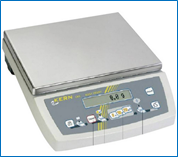
\includegraphics[scale=1.1]{bala.png}
\includegraphics[scale=1.05]{etalon.png}
\caption{La balance et les poids étalonné}
\end{center}
\end{figure}
\newpage
\textbf{\underline{Analyse de résultat du test:}}\\
* La linéarité :  

\item - $R^2$ = 0.8\% est très faible (proche de zéro)
\item - P value de la pente = 0,716 > 0,05\\
$\Longrightarrow$ Pas de linéarité. 
 \begin{figure}[!h]
\begin{center}
\includegraphics[scale=1.1]{linaa.png}
\caption{Test de linéarité}
\end{center}
\end{figure}\\


 * Bais de l’instrumentation : \\
 \item - La moyenne de bais de la balance = 0.003 
\item - P value est significative\\
$\Longrightarrow$ La balance est très précise. 
\begin{figure}[!h]
\begin{center}
\includegraphics[scale=0.7]{qui.png}
\includegraphics[scale=0.9]{bais.png}
\caption{Bais de la balance}
\end{center}
\end{figure}
 
 
\fbox{\parbox{\textwidth}{ 
\\
\textbf{Conclusion} : l'instrumentation de mesure (la balance) est non linéaire et précise, donc on peut considérer les poids des données fiables et très précis.
}}\\
 
\subsection{Étude de stabilité des accessoires}
La variation entre les pièces est un phénomène normal, mais il est très important d'étudier la stabilité de cette variation :

* entre les lots du même article

* entre des lots de différent arrivages du même article\\
Donc il faut étudier scientifiquement la stabilité de la moyenne et l'écart type.
\subsubsection{Test d'égalité de la moyenne}

Pour auditionner la différence de la moyenne, on a appliqué \textbf{t-test} et on a procédé comme suit :
\item 1- sélectionner aléatoirement deux lots d'un article (Cuir, Label, bouton, rivet et Hangtag).
\item 2- pour chaque lot, on a tiré aléatoirement un échantillon de 30 pièces.
\item 3- on a pesé ces pièces par la balance.
\item 4- à l'aide du logiciel Minitab on a appliqué le t-test.

\begin{figure}[!h]
\begin{center}
\includegraphics[scale=1.15]{ttest.png}
\caption{Exemple d'un t-test de la moyenne pour Label}
\end{center}
\end{figure}\\

\item - P value = 0,637 > 0,05\\
$\Longrightarrow$ \textbf{Pas de différence} entre les moyennes de deux lot d'un même arrivage

 on a refaire le meme test mais cette fois pour deux lots de différent arrivage on a trouvé 
\item - P value = 0,602 > 0,05\\
$\Longrightarrow$ \textbf{Pas de différence} entre les moyennes de différent arrivage 

\subsubsection{Test d'égalité de l'écart type}
Sur les mêmes échantillons on a appliqué un test d'écart type
\begin{figure}[!h]
\begin{center}
\includegraphics[scale=1]{ecaart.png}
\caption{Test de l'écart type}
\end{center}
\end{figure}\\
\item - P value = 0,638 > 0,05\\
$\Longrightarrow$ \textbf{Pas de différence} entre les écarts types du même arrivage.\\
Idem pour les lots de différent arrivage:

\item - P value = 0,701 > 0,05\\
$\Longrightarrow$ \textbf{Pas de différence} entre les écarts types de différent arrivage. \\


\fbox{\parbox{\textwidth}{ 
\\
\textbf{Conclusion} : pour tous les articles il n'y a pas de différence de moyenne et d'écart type. Ce qui implique que tous les accessoires sont stables. 
}}\\





\subsection{La formule de calcul du poids minimum}

On vise de trouver une formule en fonction de risque et nombre mentionné que nous donne un poids et qu'on est sûr qu'on est dans une zone de sécurité et que le lot n'est pas manquant.

on note:
\item $ \underline{X}( x_{i})$ : Les poids des pièces.
\item n : nombre mentionné (théorique).
\item N : nombre réel.
\item r : risque.
\item $\mu$ : moynne de l'échantillon.
\item  $\sigma$ : l'écart type de l'échantillon.
 
 
On a : $x_{i} \hookrightarrow N(\mu , \sigma^{2}) $\\

$\Longrightarrow \sum_{i=1}^{n} x_{i} \hookrightarrow N(n\mu , n\sigma^{2}) $ \\

$\Longrightarrow \overline{X} \hookrightarrow N(\mu , \frac{\sigma^{2}}{n}) $\\

On note par P le poids minimum  : \\
$\mathcal P ({ \sum_{}^{} x_{i} > N \mu}) = 1- r$\\

$\Longrightarrow \mathcal P ({ \frac{\sum_{}^{} x_{i} - n\mu}{\sigma \sqrt{n}} >\frac{N \mu - n \mu}{\sigma \sqrt{n}}}) =1- r  $\\

$\Longrightarrow  \Phi( \frac{N \mu - n \mu}{\sigma \sqrt{n}} )= 1 - r   $\\

$\Longrightarrow \frac{N \mu - n \mu}{\sigma \sqrt{n}} = \Phi^{-1}(1-r)$\\

$\Longrightarrow N \mu = \Phi^{-1}(1-r) \sigma \sqrt{n} + n \mu $\\

$\Longrightarrow P =  n \mu + \Phi^{-1}(1-r) \sigma \sqrt{n} $

    
\fbox{\parbox{\textwidth}{ 
Le poids minimum : 
\begin{equation}
    \textbf{$ P =  n \mu + \Phi^{-1}(1-r) \sigma \sqrt{n}$} \label{pp}
\end{equation}
}}

Plus bas dans l'ordre d'importance, on peut déterminer le nombre de pièce à partir de poids réel avec un risque r. On a : 

$ P =  n \mu + \Phi^{-1}(1-r) \sigma \sqrt{n} $\\

$\Longrightarrow (P - n \mu)^2 =  (\Phi^{-1}(1-r))^{2} \sigma^{2} n $\\

$\Longrightarrow n ^{2} \mu^2 - n ( 2 P \mu +(\Phi^{-1}(1-r))^{2} \sigma^{2}) + P^{2}  $\\
 L'équation est sous forme d'un produit remarquable $ a X^{2}+ b X + c $\\
 Et sachant que le nombre de pièces ne peut pas être négative donc on obtient : \\
 
\fbox{\parbox{\textwidth}{ 
Le nombre de pièces: 
\begin{equation}
\textbf{$ N =( \frac{- \sigma \Phi^{-1}(1-r)) +\sqrt{\Phi^{-1}(1-r))^{2} \sigma^{2} + 4 \mu P}  }{2 \mu})^{2} $  }  \label{nn}
\end{equation}
}}


\subsection{Expérimentation de la formule}
De la théorie à la pratique, on a passé par deux phase :
\subsubsection{Phase 1 : Détermination des paramètres} 
\item 1- Sélectionner aléatoirement un échantillon au minimum de 30 pièces. 
\item 2- Peser les pièces par la balance attentivement.
\item 3- Calculer la moyenne et l'écart type de l'échantillon.



\begin{figure}[!h]
\begin{center}
\includegraphics[scale=0.033]{a0.jpg}
\includegraphics[scale=0.033]{a1.jpg}\\
\includegraphics[scale=0.025]{a2.jpg}
\caption{Exemple pratique}
\end{center}
\end{figure}\\







\subsubsection{Phase 2 : Echantillon pour tester}
\item 4- Compter manuellement le tous les pièces le lot.
\item 5- Peser le lot net (sans emballage).
\item 6- Peser et compter des échantillons (des petits quantité).\\

 Après avoir poursuivre ce étapes, on va comparer le nombre fournis par la formule et le nombre réel. Le tableau ci-dessous récapitule un exemple du travail effectuté pour le boutons voir Tab. 4.4.\\

\begin{center}
 \includegraphics[scale=0.9]{bouton.png} 
 \includegraphics[scale=0.8]{param.PNG}
  \includegraphics[scale=0.75]{echh.PNG}
\end{center}
\begin{table}[!htbp]
\begin{center}
\caption{Exemple de boutons}
 \end{center}
\end{table}\\


Les résultats sont bons on est dans la zone de sécurité dont :
\item $ \rightarrow $  Le poids réel est toujours supérieur ou égale au poids formule avec un risque fixé.
\item  $ \rightarrow $ Le nombre de pièces réel est toujours supérieur ou égale au nombre formule.


\subsection{Mise en œuvre de la formule de calcul}
Pour SARTEX cette formule est utile sur deux volets : 
\subsubsection{Volet externe :  fournisseur}
Poue éviter la manque des pièces par le fournisseur, on va : 
\item 1- Exiger le fournisseurs à envoyer un poids supérieur ou égale au \underline{poids} déterminé par la formule avec un risque de 1 pour 1000.
\item 2- Dès la réception des accessoires, on va contrôler les quantités mentionnées par le fournisseur par rapport la quantité fournit par la formule avec un risque de 1 pour 1000.
\subsubsection{Volet interne : SARTEX}
Losqu'on est sûr que la quantité envoyé est complète et comme une étape préparative de production, le magasin des accessoires prepare des paquets d'accessoires d'un nombre bien déterminé (selon une fiche consommation reeeeeeeef************) d'ou cette étape nécessite un deuxième comptage manuel.\\


- L'idée est de connecter la balance à une application informatique, en effet l'application va convertir le poids pesé par l'employée à un nombre de pièce en utilisant la formule avec un risque de 5\%.
de cette manière l'employé va \textbf{ajouter des quantités} sur la balance jusqu'à aboutir au \textbf{nombre souhaitable}
\subsection{Mise en place d'une application informatique}

\underline{\textit{\textbf{Outil de travail :}}}\\
Pour élaborer une application informatique on va utilisé Shiny, c'est un package R développé par RStudio qui permet la création des
applications web interactives permettant de réaliser toutes les analyses disponibles
sous R. Shiny offre des extensions avancées tel que Shinydashboard
qui est un outil permettant de développer des tableaux de bord.
Nous avons utilisé le package ShinyDashboard pour développer l'application.\\

\underline{\textit{\textbf{Architecture technique de l'application :}}}
\item - L'utilisateur de l'application accède à l'application à travers un navigateur
web.
\item - Le navigateur web permet d'envoyer des données fournies par l'utilisateur et
des requêtes au serveur web.
\item - Le serveur web traite les requêtes et exécute le code de l'application, puis génère une réponse qu'il renvoie au serveur web qu'il l'enverra au navigateur web de l'utilisateur.
\begin{figure}[!h]
\begin{center} 
\includegraphics[scale=0.75]{archi.PNG} 
\caption{Architecture technique de l'application}
\end{center}
\end{figure}\\

\subsubsection{Présentation de l'application : Accessoires}
L'application contient quatre principales :
\item a- \textbf{Acceuil}
\item b- \textbf{Visualisation de données}
\item c- \textbf{Volet externe fournisseurs}
\item d- \textbf{Volet interne SARTEX}\\
 
 
 
 
 
 \textit{\textbf{1 - Acceuil :}} \\

 
 
\textit{\textbf{ 2 - Visualisation de données :}} \\
 À travers l'onglet Visualisation de données , l'utilisateur peut sur le premier plan d'importer la base .CSV en choissisant le séparateur, les quotes et l'entête.\\
 \begin{figure}[!h]
\begin{center} 
\includegraphics[scale=0.5]{appimpo} 
\caption{Importation de données}
\end{center}
\end{figure}\\
Une fois la base de données est importé, l'utilisateur peut consulter deux onglets:\\
\underline{\textbf{Résumé}}
\item - Visualiser les données : pour vérifier l'importation est bien fait.
\item - Visualiser d'un résumé de dispersion statistique de données (la moyenne, écart type,  étendue).\\

\begin{figure}[!h]
\begin{center} 
\includegraphics[scale=0.45]{appres} 
\caption{Importation de données}
\end{center}
\end{figure}


\underline{\textbf{Carte de contrôle}}
\item - Cette carte des poids pesés avec ces limites de contrôle sert à détecter des valeurs aberrantes s'ils existent. Elle très importante les problèmes de pesage qui vont fausser le calcul après.\\

\begin{figure}[!h]
\begin{center} 
\includegraphics[scale=0.7]{appcar} 
\caption{Carte de contrôle}
\end{center}
\end{figure}\\



\textit{\textbf{3 - Volet externe fournisseur :}} 

 Cette partie contient deux partie :
\item -\underline{\textbf{Poids exigé}} : permet l'utilisation d'entrer le nombre de pièces mentionnées sur le paquet et le risque et l'application affiche le poids minimum qui grantie le nombre avec le risque que vous avez déjà fixé en appliquant la formule \eqref{pp}. Elle est didiée aux fournisseurs avant d'envoyer les accesoires.



\begin{figure}[!h]
\begin{center} 
\includegraphics[scale=0.7]{apppoi.PNG} 
\caption{Poids exigé}
\end{center}
\end{figure}\\

\item - \underline{\textbf{Contrôler l'arrivage}} : permet de entrer le poids réel trouvé et nombre mentionné sur le paquet et l'application vous informe si \underline{le compte est bon ou non} avec un risque de 1 pour 1000.

\begin{figure}[!h]
\includegraphics[scale=0.57]{appvalo}\includegraphics[scale=0.57]{appvaln}
\caption{Contrôler l'arrivage}
\end{figure}\\
 
 
 
\textit{\textbf{4 - Volet interne SARTEX:}} \\

Cette Partie est didée aux employés SARTEX, qui leur permet de convertir le poids en nombre de pièces en applicant la formule \eqref{nn} 


 
 \begin{figure}[!h]
\includegraphics[scale=0.7]{appconv}\
\caption{Nombre de pièces}
\end{figure}\\
 
 
 
 















\newpage
\section*{CONCLUSION GÉNÉRALE}

\addcontentsline{toc}{section}{CONCLUSION GÉNÉRALE}
\thispagestyle{fancy}
\lhead{CONCLUSION GÉNÉRALE}


\newpage
\chapter*{Bibliographie et Webographie}
\addcontentsline{toc}{section}{Bibliographie}
\thispagestyle{fancy}
\lhead{Bibliographie}


\item AMDEC Guide pratique,Saint-Denis Cedex, 2 edition, 2007 [01]
\item Statistical quality control volume 7 . Wiley New York, 6 edition, 2009.
\item Les Fiches outils DU LEAN SIX SIGMA, Saint- Germain Paris, 1 edition, 2016. 
\item http://www.opex-management.com [9]
 \item https://www.automation-sense.com [10]
\item http://www.bluelean.fr [11]
\item https://www.piloter.org [12]

\appendix
\lhead{Annexe}


\section{Le planning}
\label{nour}
 \includegraphics[scale=0.7 , angle=90]{b.PNG}
 \begin{center}
     \includepdf[pages=1,scale=0.8 ,pagecommand={\thispagestyle{francy}\section{Charte projet}}]{m.pdf}

 \end{center}
 
\label{nour11111} 
 
 
\includepdf[pages=2, scale=0.7 ,pagecommand={\thispagestyle{francy}\section{Schématisation de processus}}]{lavv.pdf}
\label{nour11}

 \includepdf[pages=3]{tt.pdf}

 \includepdf[pages=4]{tt.pdf}
 \includepdf[pages=5]{tt.pdf}

\section{Plan de surveillance}
\label{nour111}
 \includegraphics[scale=0.775 , angle=90]{ssss.PNG}\\
 \includegraphics[scale=0.775 , angle=90]{see.PNG}\\
  \includegraphics[scale=0.85 , angle=90]{plz.PNG}
  
  
\begin{center}
    
\includepdf[pages=1,scale=0.9 ,pagecommand={\thispagestyle{francy}\section{Manuel de travail test R\&R}}]{mannou.pdf}

\label{nour1111} 

\includepdf[pages=2,scale=0.95 ,pagecommand={\thispagestyle{francy}}]{mannou.pdf}
\end{center}






\end{document}